%%%%%%%%%%%%%%%%%%%%%%%%%%%%%%%%%%%%
% Slide options
%%%%%%%%%%%%%%%%%%%%%%%%%%%%%%%%%%%%

% Option 1: Slides with solutions

\documentclass[slidestop,compress,mathserif]{beamer}
\usepackage{booktabs}
\newcommand{\soln}[1]{\textit{#1}}
\newcommand{\solnGr}[1]{#1}

% Option 2: Handouts without solutions

%\documentclass[11pt,containsverbatim,handout]{beamer}
%\usepackage{pgfpages}
%\pgfpagesuselayout{4 on 1}[letterpaper,landscape,border shrink=5mm]
%\newcommand{\soln}[1]{ }
%\newcommand{\solnGr}{ }

%%%%%%%%%%%%%%%%%%%%%%%%%%%%%%%%%%%%
% Style
%%%%%%%%%%%%%%%%%%%%%%%%%%%%%%%%%%%%
%%%%%%%%%%%%%%%%%%%%%%%%%%%%%%%%%%%%%%%%%%%%%%%%%%%%%%%%%%%%%%%%%%%%%%%%
% MA213/214 shared slide style
%
% "Calm & Cool" palette + content-type callout boxes.
% Overhauled (2026) from the original OpenIntro/metropolis style:
%   - all OpenIntro visual branding removed (logo, grid, colors)
%   - a low-key cool palette (see colors below)
%   - tcolorbox callout boxes so students recognize content types
% See common/README.md for the command cheat-sheet.
%%%%%%%%%%%%%%%%%%%%%%%%%%%%%%%%%%%%%%%%%%%%%%%%%%%%%%%%%%%%%%%%%%%%%%%%

\usetheme{metropolis}

%%%%%%%%%%%%%%%%
% Packages
%%%%%%%%%%%%%%%%

\usepackage{geometry}
\usepackage{graphicx}
\usepackage{amssymb}
\usepackage{epstopdf}
\usepackage{amsmath}  	% this permits text in eqnarray among other benefits
\usepackage{url}		% produces hyperlinks
\usepackage{hyperref}	% allows for color usage in tables
\usepackage[english]{babel}
\usepackage[latin1]{inputenc}
\usepackage{colortbl}	% allows for color usage in tables
\usepackage{multirow}	% allows for rows that span multiple rows in tables
\usepackage{color}		% this package has a variety of color options
\usepackage{pgf}
\usepackage{calc}
\usepackage{ulem}
\usepackage{multicol}
\usepackage{textcomp}
\usepackage{txfonts}
\usepackage{listings}
\usepackage{tikz}
\usepackage{array}
\usepackage{wasysym}
\usepackage{fancyvrb}
\usepackage{etoolbox}             % \ifstrempty for optional box subtitles
\usepackage[most]{tcolorbox}      % content-type callout boxes
\tcbuselibrary{listings}          % R-code block (\begin{rblock})
\usepackage{fontawesome5}         % box icons

%%%%%%%%%%%%%%%%
% Remove navigation symbols
%%%%%%%%%%%%%%%%

\setbeamertemplate{navigation symbols}{}

%%%%%%%%%%%%%%%%
% "Calm & Cool" palette
%%%%%%%%%%%%%%%%

% chrome / structure / body
\definecolor{ccSlate}{HTML}{2E3742}   % frametitle bar, structure, section pages (deep neutral slate)
\definecolor{ccInk}{HTML}{2B2B2B}     % body text
\definecolor{ccWash}{HTML}{FCF8F1}    % gentle warm title-slide background wash (complements the cool blues)

% example (blue)
\definecolor{ccBlue}{HTML}{2F6690}
\definecolor{ccBlueBg}{HTML}{EAF1F7}
% interactive activity / discussion (green)
\definecolor{ccGreen}{HTML}{4E8A6B}
\definecolor{ccGreenBg}{HTML}{E9F3EC}
% solution (purple)
\definecolor{ccPurple}{HTML}{6F5499}
\definecolor{ccPurpleBg}{HTML}{EFEAF6}
% worksheet / focused work (terracotta)
\definecolor{ccTerra}{HTML}{C2693E}
\definecolor{ccTerraBg}{HTML}{FAEDE4}
% formula / definition (neutral slate)
\definecolor{ccGray}{HTML}{5C6B7A}
\definecolor{ccGrayBg}{HTML}{EEF1F4}
% caution / common pitfall (brick red)
\definecolor{ccRed}{HTML}{B23A48}
\definecolor{ccRedBg}{HTML}{FAEAEC}
% key idea / takeaway (muted gold)
\definecolor{ccGold}{HTML}{9C7A28}
\definecolor{ccGoldBg}{HTML}{F7F1DF}
% learning goals / lesson outcomes (teal)
\definecolor{ccTeal}{HTML}{2C6E6B}
\definecolor{ccTealBg}{HTML}{E6F0EF}
% learning objectives (indigo)
\definecolor{ccIndigo}{HTML}{45507A}
\definecolor{ccIndigoBg}{HTML}{ECEEF4}
% R code / output (gray)
\definecolor{ccCode}{HTML}{5F5E5A}
\definecolor{ccCodeBg}{HTML}{F4F5F6}

% neutral grays kept from the original style
\definecolor{gray}{rgb}{0.5, 0.5, 0.5}
\definecolor{darkGray}{rgb}{0.3, 0.3, 0.3}
\definecolor{darkerGray}{rgb}{0.2, 0.2, 0.2}

% Backwards-compatible aliases: old OpenIntro color names now point at the
% new palette, so existing \textcolor{oiB}{...}, \hl{...}, etc. keep working.
\colorlet{oiB}{ccBlue}
\colorlet{oiG}{ccGreen}
\colorlet{hlblue}{ccBlue}
\colorlet{rubineRed}{ccRed}
\colorlet{irishGreen}{ccGreen}
\colorlet{lightGreen}{ccGreen}

%%%%%%%%%%%%%%%%
% Restyle metropolis with the Calm & Cool chrome
%%%%%%%%%%%%%%%%

\metroset{block=fill}

\setbeamercolor{normal text}{fg=ccInk, bg=white}
\setbeamercolor{structure}{fg=ccSlate}
\setbeamercolor{alerted text}{fg=ccBlue}
\setbeamercolor{example text}{fg=ccGreen}
\setbeamercolor{frametitle}{bg=ccSlate, fg=white}
\setbeamercolor{progress bar}{fg=ccBlue}
\setbeamercolor{title separator}{fg=ccBlue}
\setbeamercolor{title}{fg=ccSlate}
\setbeamercolor{subtitle}{fg=ccBlue}
\setbeamercolor{author}{fg=ccInk}
\setbeamercolor{institute}{fg=ccGray}
\setbeamercolor{date}{fg=ccGray}
\setbeamercolor{section title}{fg=ccSlate}
\setbeamercolor{standout}{fg=white, bg=ccSlate}

% Section pages sit on the same warm wash as the title slide. We keep
% metropolis's section-title styling and just paint a full-page ccWash
% background behind it (needs >=2 pdflatex passes for the current-page node).
\setbeamertemplate{section page}{%
  \begin{tikzpicture}[remember picture, overlay]
    \fill[ccWash] (current page.south west) rectangle (current page.north east);
  \end{tikzpicture}%
  \centering
  \begin{minipage}{22em}
    \raggedright
    \usebeamercolor[fg]{section title}%
    \usebeamerfont{section title}%
    \insertsectionhead\\[-1ex]
    \usebeamertemplate*{progress bar in section page}%
    \par
  \end{minipage}\par
  \vspace{\baselineskip}
}

%%%%%%%%%%%%%%%%
% Custom inline text commands (recolored to the palette)
%%%%%%%%%%%%%%%%

% degree
\newcommand{\degree}{\ensuremath{^\circ}}

% cite
\newcommand{\ct}[1]{
\vfill
{\tiny #1}}

\newcommand{\NamedNote}[2]{
\rule{2.5cm}{0.25pt} \\ \textit{\footnotesize{\textcolor{rubineRed}{#1:} \textcolor{darkerGray}{#2}}}}

% Note
\newcommand{\Note}[1]{
\rule{2.5cm}{0.25pt} \\ \textit{\footnotesize{\textcolor{rubineRed}{Note:} \textcolor{darkerGray}{#1}}}}

% Remember
\newcommand{\Remember}[1]{\textit{\scriptsize{\textcolor{ccTerra}{Remember:} #1}}}

% expected counts
\newcommand{\ex}[1]{\textit{\textcolor{ccBlue}{#1}}}

% red
\newcommand{\red}[1]{\textit{\textcolor{rubineRed}{#1}}}

% pink
\newcommand{\pink}[1]{\textit{\textcolor{rubineRed!90!white!50}{#1}}}

% green
\newcommand{\green}[1]{\textit{\textcolor{irishGreen}{#1}}}

% orange
\newcommand{\orange}[1]{\textit{\textcolor{ccTerra}{#1}}}

% links: webURL, webLink, appLink
\newcommand{\webURL}[1]{\urlstyle{same}{ \textit{\textcolor{darkGray}{\url{#1}}}}}
\newcommand{\webLink}[2]{\href{#1}{\textcolor{darkGray}{{#2}}}}
\newcommand{\appLink}[2]{\href{#1}{\textcolor{white}{{#2}}}}

% mail
\newcommand{\mail}[1]{\href{mailto:#1}{\textit{\textcolor{darkGray}{#1}}}}

% highlighting: hl, hlGr, mathhl
\newcommand{\hl}[1]{\textit{\textcolor{hlblue}{#1}}}
\newcommand{\hlGr}[1]{\textit{\textcolor{lightGreen}{#1}}}
\newcommand{\mathhl}[1]{\textcolor{hlblue}{\ensuremath{#1}}}

%%%%%%%%%%%%%%%%
% Structural helpers (unchanged from the original)
%%%%%%%%%%%%%%%%

% two col: two columns
\newenvironment{twocol}[4]{
\begin{columns}[c]
\column{#1\textwidth}
#3
\column{#2\textwidth}
#4
\end{columns}
}

% slot (for probability calculations)
\newenvironment{slot}[2]{
\begin{array}{c}
\underline{#1} \\
#2
\end{array}
}

% pr: left and right parentheses
\newcommand{\pr}[1]{
\left( #1 \right)
}

% cancel
\newcommand{\cancel}[1]{%
    \tikz[baseline=(tocancel.base)]{
        \node[inner sep=0pt,outer sep=0pt] (tocancel) {#1};
        \draw[red, line width=0.5mm] (tocancel.south west) -- (tocancel.north east);
    }%
}

% removepagenumbers
\newcommand{\removepagenumbers}{%
  \setbeamertemplate{footline}{}
}

% change margin
\newenvironment{changemargin}[2]{%
\begin{list}{}{%
\setlength{\topsep}{0pt}%
\setlength{\leftmargin}{#1}%
\setlength{\rightmargin}{#2}%
\setlength{\listparindent}{\parindent}%
\setlength{\itemindent}{\parindent}%
\setlength{\parsep}{\parskip}%
}%
\item}{\end{list}}

% footnote
\long\def\symbolfootnote[#1]#2{\begingroup%
\def\thefootnote{\fnsymbol{footnote}}\footnote[#1]{#2}\endgroup}

% commands from the book
\newenvironment{data}[1]{\texttt{#1}}{}
\newenvironment{var}[1]{\texttt{#1}}{}
\newenvironment{resp}[1]{\texttt{#1}}{}

%%%%%%%%%%%%%%%%
% Content-type callout boxes (tcolorbox)
%
% Each type has a colored title strip (icon + label) over a light fill.
% Color = content type; the label + icon reinforce it (so the cue does
% not rely on color alone).
%%%%%%%%%%%%%%%%

\tcbset{
  cccallout/.style 2 args={
    enhanced, breakable=false,
    colback=#2, colframe=#1, colbacktitle=#1, coltitle=white,
    fonttitle=\bfseries\footnotesize,
    boxrule=0.6pt, arc=2.5pt, outer arc=2.5pt,
    left=5pt, right=5pt, top=3pt, bottom=3pt, boxsep=2pt,
    toptitle=2pt, bottomtitle=2pt, lefttitle=5pt,
    before skip=5pt, after skip=5pt,
  },
}

% One-off / collection of examples (blue): \workedexample[subtitle]{body}.
% (Named \workedexample, not \example, because beamer defines \example.)
\newtcolorbox{examplebox}[1][]{cccallout={ccBlue}{ccBlueBg},
  title={\faIcon{lightbulb}~~Example\ifstrempty{#1}{}{ \textmd{---}\ #1}}}
\newcommand{\workedexample}[2][]{\begin{examplebox}[#1]#2\end{examplebox}}

% Running-example header (blue): \examplehead{name} at the top of each frame of a
% multi-slide running example. A one-off or a collection of examples uses the
% \workedexample box above instead.
\newcommand{\examplehead}[1]{%
  \vspace{-0.4em}\par\noindent\tcbox[on line, colback=ccBlue, colframe=ccBlue, coltext=white,
    boxrule=0pt, arc=2pt, left=5pt, right=5pt, top=1pt, bottom=1pt,
    box align=base, nobeforeafter]{\footnotesize\bfseries\faIcon{lightbulb}\,Running example}%
  \ifstrempty{#1}{}{\enspace{\footnotesize\bfseries\textcolor{ccBlue}{#1}}}%
  \par\nobreak\vspace{-0.6em}{\color{ccBlue}\rule{\linewidth}{0.7pt}}\par\nobreak\vspace{-0.8em}}

% Interactive activity (green): \activity[subtitle]{body}
\newtcolorbox{activitybox}[1][]{cccallout={ccGreen}{ccGreenBg},
  title={\faIcon{users}~~Activity\ifstrempty{#1}{}{ #1}}}
\newcommand{\activity}[2][]{\begin{activitybox}[#1]#2\end{activitybox}}

% Discussion question (green): \dq{body}
\newtcolorbox{dqbox}{cccallout={ccGreen}{ccGreenBg}, title={\faIcon{comments}~~Discussion}}
\newcommand{\dq}[1]{\begin{dqbox}#1\end{dqbox}}

% Solution (purple): \solnbox{body}. Gated by the per-deck \soln toggle, so it
% shows in the instructor build and vanishes from the student handout build.
% (Named \solnbox, not \solution, because beamer already defines \solution.)
\newtcolorbox{solutionbox}{cccallout={ccPurple}{ccPurpleBg}, title={\faIcon{key}~~Solution}}
\newcommand{\solnbox}[1]{\soln{\begin{solutionbox}#1\end{solutionbox}}}

% Worksheet / focused work (terracotta): \worksheet[subtitle]{body}
\newtcolorbox{worksheetbox}[1][]{cccallout={ccTerra}{ccTerraBg},
  title={\faIcon{pencil-alt}~~Worksheet\ifstrempty{#1}{}{ #1}}}
\newcommand{\worksheet}[2][]{\begin{worksheetbox}[#1]#2\end{worksheetbox}}

% Formula / definition (neutral slate). Supports both real usages found in the
% decks: \formula{title}{body} and the bare \formula{body} (title defaults to
% "Formula"). The second group is an optional brace argument.
\newtcolorbox{formulabox}[1][Formula]{cccallout={ccGray}{ccGrayBg},
  title={\faIcon{square-root-alt}~~#1}}
\NewDocumentCommand{\formula}{m g}{%
  \IfNoValueTF{#2}%
    {\begin{formulabox}#1\end{formulabox}}%
    {\begin{formulabox}[#1]#2\end{formulabox}}}

% Common pitfall / caution (brick red): \caution[subtitle]{body}
\newtcolorbox{cautionbox}[1][]{cccallout={ccRed}{ccRedBg},
  title={\faIcon{exclamation-triangle}~~Caution\ifstrempty{#1}{}{ #1}}}
\newcommand{\caution}[2][]{\begin{cautionbox}[#1]#2\end{cautionbox}}

% Key idea / takeaway (muted gold): \keyidea[subtitle]{body}
\newtcolorbox{keyideabox}[1][]{cccallout={ccGold}{ccGoldBg},
  title={\faIcon{star}~~Key idea\ifstrempty{#1}{}{ #1}}}
\newcommand{\keyidea}[2][]{\begin{keyideabox}[#1]#2\end{keyideabox}}

% Learning goals / lesson outcomes (teal): \goals{body}. Sits under the short
% LO headings on the objectives slide; body is the "you should be able to" list.
\newtcolorbox{goalsbox}{cccallout={ccTeal}{ccTealBg}, fontupper=\footnotesize,
  top=1pt, bottom=2pt, boxsep=1pt, before skip=3pt,
  title={\faIcon{bullseye}~~By the end of today, you should be able to\ldots}}
\newcommand{\goals}[1]{\begin{goalsbox}#1\end{goalsbox}}

% Learning objectives (indigo): \objectives{body} -- the formal LO headings,
% shown alongside \goals on the objectives slide.
\newtcolorbox{objectivesbox}{cccallout={ccIndigo}{ccIndigoBg}, fontupper=\small,
  top=1pt, bottom=2pt, boxsep=1pt, before skip=3pt,
  title={\faIcon{clipboard-list}~~Learning objectives}}
\newcommand{\objectives}[1]{\begin{objectivesbox}#1\end{objectivesbox}}

% Defaults for a bare \begin{lstlisting}. Without these it inherits the listings
% package defaults: 11pt type, fixed-width columns (which spaces code out as
% "a g e _ f i t"), and no line breaking, so a long line silently runs off the
% right edge of the slide. A deck that passes its own basicstyle still wins.
% Layout only -- syntax coloring is left to the \begin{rblock} environment.
\lstset{
  basicstyle=\ttfamily\footnotesize, columns=fullflexible,
  breaklines=true, breakindent=1.5em, showstringspaces=false,
  numbers=none, frame=none}

% R code / output (gray): \begin{rblock}[subtitle] ... \end{rblock}
% NOTE: a frame containing an rblock must be declared \begin{frame}[fragile].
\lstdefinestyle{ccR}{
  language=R, basicstyle=\ttfamily\footnotesize, columns=fullflexible,
  breaklines=true, showstringspaces=false, numbers=none, frame=none,
  keywordstyle=\color{ccBlue}, commentstyle=\color{ccGreen!75!black},
  stringstyle=\color{ccTerra}}
\newtcblisting{rblock}[1][]{cccallout={ccCode}{ccCodeBg},
  title={\faIcon{terminal}~~R\ifstrempty{#1}{}{ #1}},
  listing only, listing style=ccR}

% --- Legacy boxes (kept so existing decks compile) ---

% app: application exercise -> alias of activity
\newcommand{\app}[1]{\activity{#1}}

% pq: practice question (green, interactive family)
\newtcolorbox{pqbox}{cccallout={ccGreen}{ccGreenBg}, title={\faIcon{list-ol}~~Practice}}
\newcommand{\pq}[1]{\begin{pqbox}#1\end{pqbox}}

% solnMult: solutions for multiple-choice practice questions (uses \soln toggle)
\newcommand{\solnMult}[1]{
\item[] \vspace{-0.59cm}
\only<1>{\item #1}
\soln{\only<2->{\item \orange{#1}}}
}

%%%%%%%%%%%%%%%%
% De-branded title frame + attribution
%%%%%%%%%%%%%%%%

% Eyebrow line on the title slide; a deck may \renewcommand this.
\newcommand{\coursetag}{MA214: Applied Statistics}

% Attribution: all slides released under CC BY-SA, crediting both the
% instructor (later material) and OpenIntro (basis of the earlier material).
\newcommand{\courseattribution}{%
  Slides by Jonathan H.~Huggins, building on materials from OpenIntro's
  \emph{Introduction to Modern Statistics} (Mine \c{C}etinkaya-Rundel et al.).
  Released under the
  \webLink{http://creativecommons.org/licenses/by-sa/3.0/us/}{CC BY-SA license}.
  Some images included under fair use (educational purposes).}

% \maketitleframe: de-branded title slide (no logo, no grid). Uses the deck's
% \title, \subtitle, and \coursetag.
\newcommand{\maketitleframe}{%
  \addtocounter{framenumber}{-1}%
  {\removepagenumbers
  \setbeamercolor{background canvas}{bg=ccWash}%
  \begin{frame}[plain]
    \vspace*{2.6em}
    {\color{ccSlate}\rule{\textwidth}{2.5pt}}\par\vspace{1.5em}
    {\usebeamerfont{date}\scshape\color{ccGray}\coursetag}\par\vspace{0.55em}
    {\usebeamerfont{title}\color{ccSlate}\inserttitle\par}
    \vspace{0.45em}{\color{ccBlue}\rule{3em}{2.5pt}}\par\vspace{0.7em}
    {\usebeamerfont{subtitle}\color{ccBlue}\insertsubtitle\par}
    \vfill
    {\color{ccGray!55}\rule{\textwidth}{0.4pt}}\par\vspace{0.45em}
    {\tiny\color{ccGray}\courseattribution\par}
    \vspace*{0.4em}
  \end{frame}}}

%%%%%%%%%%%%%%%%
% Graphics
%%%%%%%%%%%%%%%%

\DeclareGraphicsRule{.tif}{png}{.png}{`convert #1 `dirname #1`/`basename #1 .tif`.png}

\graphicspath{ {../../common/} {figures/}  }


%%%%%%%%%%%%%%%%%%%%%%%%%%%%%%%%%%%%
% Preamble
%%%%%%%%%%%%%%%%%%%%%%%%%%%%%%%%%%%%

\title[Lecture 14]{Lecture 14: Inference for multiple regression}
\subtitle{Module 3: Regression Inference}
\author{Introduction to Modern Statistics, 2nd Edition}
\institute{$\:$ \\ {\footnotesize Based on slides developed by Mine \c{C}etinkaya-Rundel of OpenIntro.  \\
The slides may be copied, edited, and/or shared via the \webLink{http://creativecommons.org/licenses/by-sa/3.0/us/}{CC BY-SA license.} \\
Some images may be included under fair use guidelines (educational purposes).}}
\date{}

%%%%%%%%%%%%%%%%%%%%%%%%%%%%%%%%%%%%
% Begin document
%%%%%%%%%%%%%%%%%%%%%%%%%%%%%%%%%%%%

\begin{document}


%%%%%%%%%%%%%%%%%%%%%%%%%%%%%%%%%%%%
% Title page
%%%%%%%%%%%%%%%%%%%%%%%%%%%%%%%%%%%%

\maketitleframe

% !TEX root =  Lecture14.tex


%%%%%%%%%%%%%%%%%%%%%%%%%%%%%%%%%%%%
% Recap/Agenda
%%%%%%%%%%%%%%%%%%%%%%%%%%%%%%%%%%%%
\begin{frame}
\frametitle{Module 3: Regression Inference}
    \begin{itemize}
        \item \hl{Previously:} inference about \emph{one} slope: the two roads, a bootstrap interval, LINE (Lecture 13).
        \item \hl{This time:} \hl{many predictors at once}. That slope test becomes one \emph{row} of an \texttt{lm()} table.
          \begin{itemize}
              \item reading the output: $\mathrm{df} = n-p-1$, every slope \emph{holding the others fixed};
              \item what \hl{multicollinearity} does to those SEs, $p$-values and intervals;
              \item when the conditions fail: \hl{transformations}, and reading a log model;
              \item \hl{interaction} terms.
          \end{itemize}
        \item \hl{Reading:} IMS Ch.\ 25.1--25.2, plus the non-linear and interaction supplements.
        \item \hl{Homework:} the assigned reading.
    \end{itemize}
\end{frame}


%%%%%%%%%%%%%%%%%%%%%%%%%%%%%%%%%%%%
% Learning objectives:
%%%%%%%%%%%%%%%%%%%%%%%%%%%%%%%%%%%%
\begin{frame}
    \frametitle{Lecture Objectives}
    \goals{%
    \begin{itemize}
    \item read a multiple regression coefficient table, and test $H_0:\beta_j=0$ against $t_{n-p-1}$;
    \item interpret each $\hat\beta_j$ \emph{holding the other predictors fixed}, and say why every row is conditional on the rest of the model;
    \item explain what \hl{collinear} predictors do to the inference, and why they leave prediction untouched;
    \item diagnose a failing model, \hl{transform} it, and interpret a $\log(y)$, $\log(x)$ or log--log coefficient;
    \item fit and read an \hl{interaction}: what $\hat\beta_3$ means when one slope depends on another predictor.
    \end{itemize}}
\end{frame}


%%%%%%%%%%%%%%%%%%%%%%%%%%%%%%%%%%%%
\begin{frame}
    \frametitle{Lecture Objectives}
    \objectives{%
    \begin{itemize}
    \item \textbf{(M3, LO3)} Interpreting Software Output for Multiple Regression
    \item \textbf{(M3, LO4)} Building and Interpreting Non-linear and Interaction Models
    \end{itemize}}
    \vspace{0.3em}
    {\small Also revisited, in the light of \emph{inference}:}
    \objectives{%
    \begin{itemize}
    \item \textbf{(M3, LO2)} Model Checking and Remedial Measures: the transformations of Lecture 13, now as model \emph{building}
    \item \textbf{(M1, LO3)} Using Regression Models: multicollinearity, from Lecture 7
    \end{itemize}}
\end{frame}



%%%%%%%%%%%%%%%%%%%%%%%%%%%%%%%%%%%%%%%%%%%%%%%%%%%%%%%%%%%%%%%%%%%%%%%%
\section{The model we can already fit}
%%%%%%%%%%%%%%%%%%%%%%%%%%%%%%%%%%%%%%%%%%%%%%%%%%%%%%%%%%%%%%%%%%%%%%%%
\begin{frame}
\frametitle{We can fit it; we cannot yet judge it}

Since Lecture 5 we have been \emph{fitting} models with several predictors: reading coefficients, adding indicator variables, comparing with $R^2_{\text{adj}}$ and AIC, worrying about collinearity.

\pause
\vspace{0.4em}
What we have never once done is ask whether any of those coefficients is \hl{real}, whether a slope we read off the table could have come from a world in which that predictor does nothing at all.

\pause
\vspace{0.4em}
Lecture 13 answered that question for \emph{one} slope. \hl{Today: all of them at once.}

\end{frame}


%%%%%%%%%%%%%%%%%%%%%%%%%%%%%%%%%%%%%%%%%%%%%%%%%%%%%%%%%%%%%%%%%%%%%%%%
\begin{frame}
\frametitle{What makes a planet big?}

The \hl{NASA Exoplanet Archive}: every confirmed planet with \emph{both} a measured mass and a measured radius: $1{,}491$ of them, $n = 890$ complete on everything we need.

\pause
\vspace{0.4em}
\hl{Response:} \texttt{planet\_radius} (Earth radii). \hl{Candidate predictors:}
{\small
\begin{itemize}
\item \texttt{planet\_mass}: the planet's mass (Earth masses)
\item \texttt{stellar\_mass}: its host star's mass (solar masses)
\item \texttt{equilibrium\_temp}: how hot the planet is (K)
\item \texttt{eccentricity}: how elliptical its orbit is
\end{itemize}}

\pause
Four predictors, one response, and \emph{no experiment}. Which of them matter?

\end{frame}


%%%%%%%%%%%%%%%%%%%%%%%%%%%%%%%%%%%%%%%%%%%%%%%%%%%%%%%%%%%%%%%%%%%%%%%%
\begin{frame}
\frametitle{Each predictor on its own}

\begin{center}
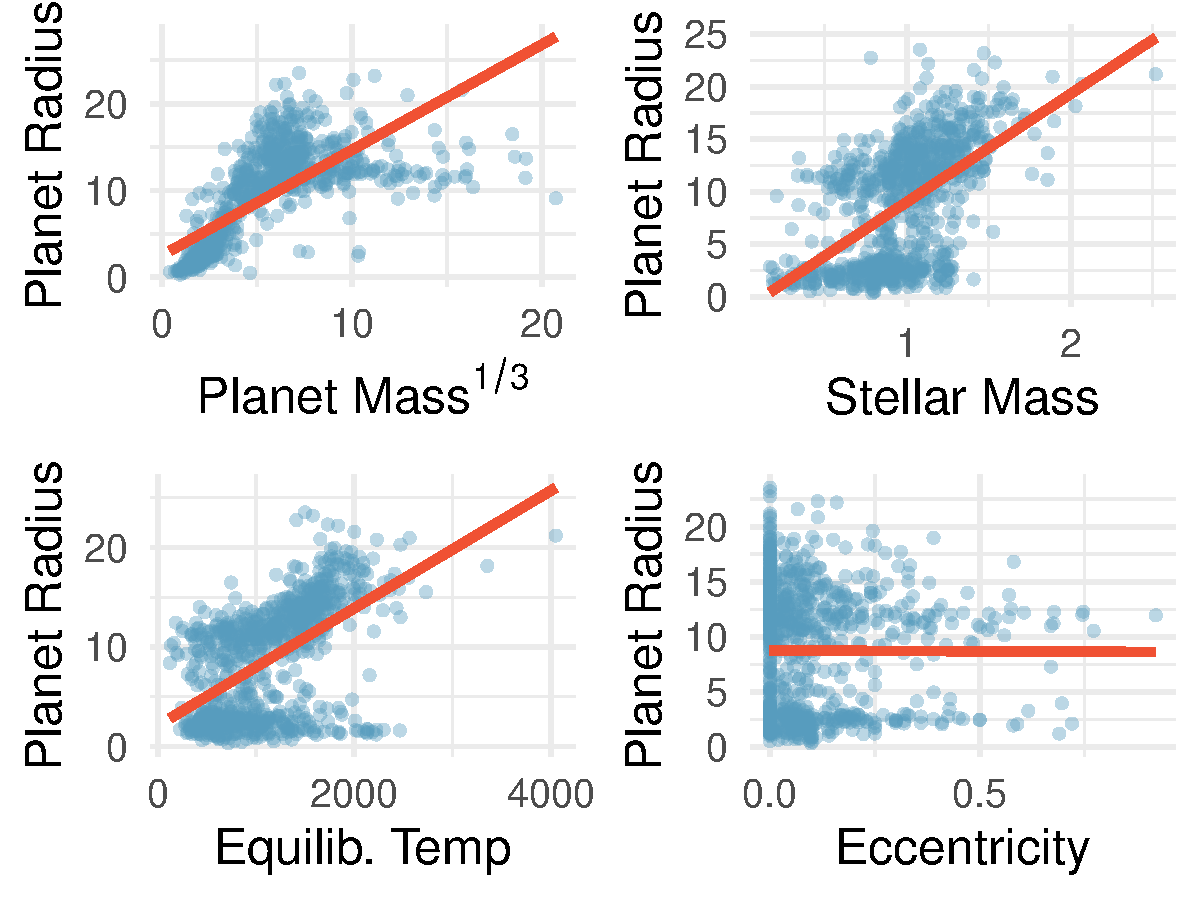
\includegraphics[width=0.62\textwidth]{pairwise_predictors.pdf}
\end{center}

\pause
\vspace{-0.3em}
{\small Mass explains the most ($R^2 = 0.52$), eccentricity essentially nothing ($R^2 = 0.00$). But four \emph{separate} regressions cannot show what each predictor adds \emph{on top of} the others.}

\end{frame}


%%%%%%%%%%%%%%%%%%%%%%%%%%%%%%%%%%%%%%%%%%%%%%%%%%%%%%%%%%%%%%%%%%%%%%%%
\begin{frame}
\frametitle{A predictor the physics hands us}

A ball of uniform density has $\text{mass} \propto \text{radius}^3$, so $\text{radius} \propto \text{mass}^{1/3}$. Regress radius on $\texttt{planet\_mass}^{1/3}$, not on raw mass:

\vspace{0.1em}
\twocol{0.5}{0.5}
{
\begin{center}
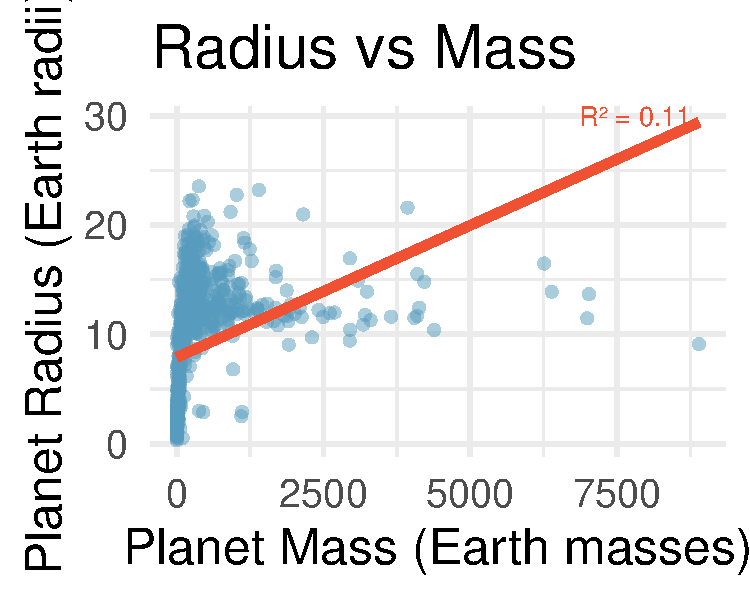
\includegraphics[width=0.92\textwidth]{exoplanet_scatter.pdf}
\end{center}
}
{
\begin{center}
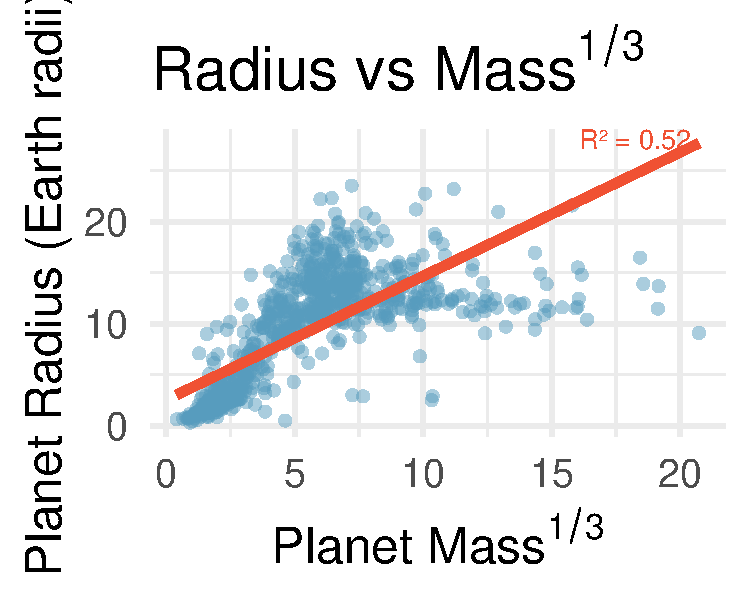
\includegraphics[width=0.92\textwidth]{exoplanet_scatter_cbrt.pdf}
\end{center}
}

\pause
\vspace{-0.2em}
{\small The cube root straightens the curve and lifts $R^2$ from $0.11$ to $0.52$: \hl{a transformation motivated by theory, not by a residual plot}. How to \emph{choose} one: second half.}

\end{frame}


%%%%%%%%%%%%%%%%%%%%%%%%%%%%%%%%%%%%%%%%%%%%%%%%%%%%%%%%%%%%%%%%%%%%%%%%
\section{Reading the software output}
%%%%%%%%%%%%%%%%%%%%%%%%%%%%%%%%%%%%%%%%%%%%%%%%%%%%%%%%%%%%%%%%%%%%%%%%
\begin{frame}
\frametitle{From one slope to many}

The model is Lecture 5's, unchanged:
$$y_i = \beta_0 + \beta_1 x_{i1} + \beta_2 x_{i2} + \cdots + \beta_p x_{ip} + \varepsilon_i.$$

\pause
\vspace{0.4em}
The \emph{inference} is Lecture 13's, unchanged, except that \texttt{lm()} now returns \hl{one row per coefficient}, each with its own estimate, standard error, $t$, $p$-value and interval.

\pause
\vspace{0.4em}
\hl{Today is those two facts, put together.} Only one number in the whole apparatus actually changes.

\end{frame}


%%%%%%%%%%%%%%%%%%%%%%%%%%%%%%%%%%%%%%%%%%%%%%%%%%%%%%%%%%%%%%%%%%%%%%%%
\begin{frame}
\frametitle{The one number that changes}

\formula{Notation}{$p$ is the number of \emph{predictors}, not counting the intercept. Fitting the model spends $p+1$ estimated numbers, so the residual degrees of freedom are $$\mathrm{df} = n - p - 1.$$}

\pause
\vspace{0.4em}
Set $p = 1$ and you get back Lecture 13's $n-2$: a line costs two numbers, a slope and an intercept. Each extra predictor costs one more.

\pause
\vspace{0.3em}
{\small For the exoplanet model below, $n = 890$ and $p = 4$, so $\mathrm{df} = 885$, and with that many the $t$ is all but a $z$. The df matters most when $n$ is small.}

\end{frame}


%%%%%%%%%%%%%%%%%%%%%%%%%%%%%%%%%%%%%%%%%%%%%%%%%%%%%%%%%%%%%%%%%%%%%%%%
\begin{frame}[fragile]
\frametitle{The fitted model}

\begin{Verbatim}[fontsize=\scriptsize]
fit <- lm(planet_radius ~ I(planet_mass^(1/3)) + stellar_mass
                          + equilibrium_temp + eccentricity,
          data = exo)
fit |> tidy()
\end{Verbatim}

\pause
\vspace{0.2em}
\begin{Verbatim}[fontsize=\scriptsize]
  term                 estimate  std.error  statistic  p.value
  (Intercept)           -1.479     0.396      -3.73     <0.001
  cbrt_mass              0.974     0.039      24.68     <0.001
  stellar_mass           2.566     0.548       4.68     <0.001
  equilibrium_temp       0.0026    0.0003      8.16     <0.001
  eccentricity          -1.646     0.885      -1.86      0.063
\end{Verbatim}

\pause
\vspace{0.2em}
{\small $n = 890$, $p = 4$, so $\mathrm{df} = 890 - 4 - 1 = 885$.}

\end{frame}


%%%%%%%%%%%%%%%%%%%%%%%%%%%%%%%%%%%%%%%%%%%%%%%%%%%%%%%%%%%%%%%%%%%%%%%%
\begin{frame}
\frametitle{What a coefficient means now}

\keyidea[-- recall, Lecture 5]{$\hat\beta_j$ is the expected change in $y$ for a one-unit increase in $x_j$ \hl{while every other predictor is held fixed}: the effect of $x_j$ \emph{net of the others}, and not the effect of regressing $y$ on $x_j$ alone. \hl{New today:} that number comes with a standard error, so we can ask how much of it is signal.}

\pause
\vspace{0.4em}
{\small
\textbf{$\texttt{mass}^{1/3}$:} $\hat\beta_1 = 0.974$, 95\% CI $(0.896,\ 1.051)$. One more unit of $\text{mass}^{1/3}$ buys about one more Earth radius, \emph{for two planets around equally massive stars, at the same temperature and eccentricity}.

\smallskip
\textbf{\texttt{stellar\_mass}:} $\hat\beta_2 = 2.57$, 95\% CI $(1.49,\ 3.64)$. A star one solar mass heavier hosts planets about $2.6$ Earth radii larger, \emph{at equal planet mass, temperature and eccentricity}.}

\end{frame}


%%%%%%%%%%%%%%%%%%%%%%%%%%%%%%%%%%%%%%%%%%%%%%%%%%%%%%%%%%%%%%%%%%%%%%%%
\begin{frame}
\frametitle{Testing and bounding one coefficient}

Everything from Lecture 13 carries over, one row at a time. To ask whether $x_j$ earns its place:
$$H_0: \beta_j = 0 \qquad\text{(with the other predictors in the model)}$$

\pause
\vspace{0.3em}
\hl{The statistic} is the estimate in units of its own noise, and the model for it is a $t$:
$$T = \frac{\hat\beta_j}{\mathrm{SE}(\hat\beta_j)} \;\sim\; t_{\,n-p-1}$$

\pause
\vspace{0.3em}
\hl{The interval} is the estimate give or take a few standard errors:
$$\hat\beta_j \pm t^\ast_{\,n-p-1}\,\mathrm{SE}(\hat\beta_j), \qquad t^\ast_{885} = 1.963$$

\pause
\vspace{0.2em}
{\small Same recipe, same table, only the degrees of freedom changed.}

\end{frame}


%%%%%%%%%%%%%%%%%%%%%%%%%%%%%%%%%%%%%%%%%%%%%%%%%%%%%%%%%%%%%%%%%%%%%%%%
\begin{frame}[fragile]
\frametitle{The intervals, straight from the table}

\begin{Verbatim}[fontsize=\scriptsize]
fit |> tidy(conf.int = TRUE)

  term                 estimate  p.value   conf.low  conf.high
  (Intercept)           -1.479    <0.001    -2.256     -0.701
  cbrt_mass              0.974    <0.001     0.896      1.051
  stellar_mass           2.566    <0.001     1.489      3.642
  equilibrium_temp       0.0026   <0.001     0.0020     0.0032
  eccentricity          -1.646     0.063    -3.383      0.091
\end{Verbatim}

\pause
\vspace{0.2em}
\dq{Three predictors have $p < 0.001$. Eccentricity has $p = 0.063$, and an interval that just barely covers zero. What should we do with it?}

\end{frame}


%%%%%%%%%%%%%%%%%%%%%%%%%%%%%%%%%%%%%%%%%%%%%%%%%%%%%%%%%%%%%%%%%%%%%%%%
\begin{frame}
\frametitle{The borderline predictor: discussion}

\emph{Eccentricity: $\hat\beta = -1.65$, $p = 0.063$, 95\% CI $(-3.38,\ 0.09)$. What should we do with it?}

\pause
\vspace{0.5em}
\solnbox{%
\begin{itemize}\setlength{\itemsep}{1pt}
\item $p = 0.063$ is weak evidence, not evidence of \emph{no} effect. The interval still allows a fairly large negative effect.
\item $890$ planets do not pin eccentricity down.
\item Do \emph{not} delete the row for missing $0.05$. ``Not significant'' describes our \emph{evidence}, not the planets.
\end{itemize}}

\end{frame}


%%%%%%%%%%%%%%%%%%%%%%%%%%%%%%%%%%%%%%%%%%%%%%%%%%%%%%%%%%%%%%%%%%%%%%%%
\begin{frame}
\frametitle{Every row is a conditional claim}

\caution{Each row tests $\beta_j = 0$ \hl{given the other predictors already in the model}. Change the model and the row changes: a predictor significant on its own can go insignificant once a relative joins it, and the reverse happens too. There is no such thing as ``the'' $p$-value of a predictor.}

\pause
\vspace{0.4em}
So the coefficient table is not a ranking of the predictors. It is a set of answers to $p$ separate questions, each of them beginning \emph{``given the rest of this model\ldots''}

\pause
\vspace{0.4em}
Which raises the obvious worry: \hl{what if two predictors are telling us the same thing?}

\end{frame}


%%%%%%%%%%%%%%%%%%%%%%%%%%%%%%%%%%%%%%%%%%%%%%%%%%%%%%%%%%%%%%%%%%%%%%%%
\section{Multicollinearity in the coefficient table}
%%%%%%%%%%%%%%%%%%%%%%%%%%%%%%%%%%%%%%%%%%%%%%%%%%%%%%%%%%%%%%%%%%%%%%%%
\begin{frame}
\frametitle{Multicollinearity, revisited}

\twocol{0.5}{0.5}
{
\begin{center}
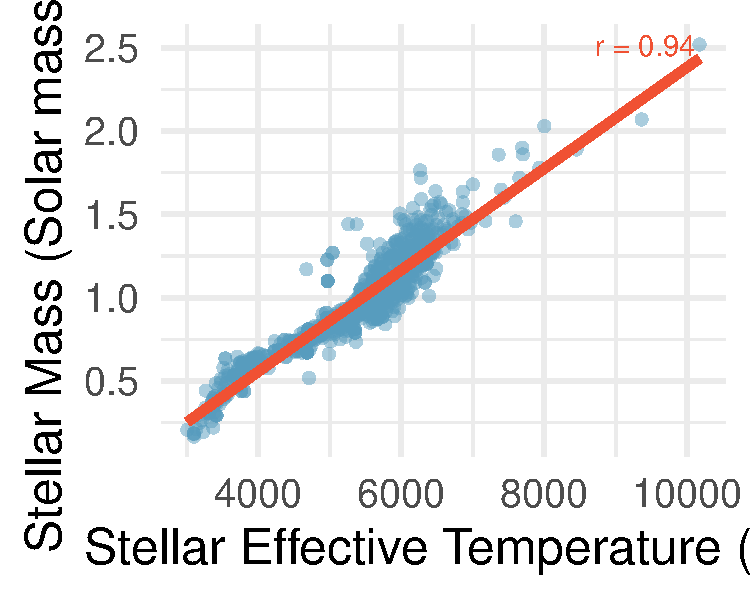
\includegraphics[width=\textwidth]{stellar_corr.pdf}
\end{center}
}
{
Heavy stars are hot stars: in these $890$ systems \texttt{stellar\_mass} and \texttt{stellar\_temp} correlate at $r = 0.94$ (VIF $= 8.2$).

\vspace{0.6em}
\hl{Lecture 7:} what collinearity \emph{is}, and how to spot it.

\vspace{0.4em}
\hl{Today:} what it does to the \emph{inference}, to the standard errors, $p$-values and intervals.
}

\end{frame}


%%%%%%%%%%%%%%%%%%%%%%%%%%%%%%%%%%%%%%%%%%%%%%%%%%%%%%%%%%%%%%%%%%%%%%%%
\begin{frame}
\frametitle{It widens the interval, not the error}

\begin{columns}[T]
\begin{column}{0.46\textwidth}
\begin{center}
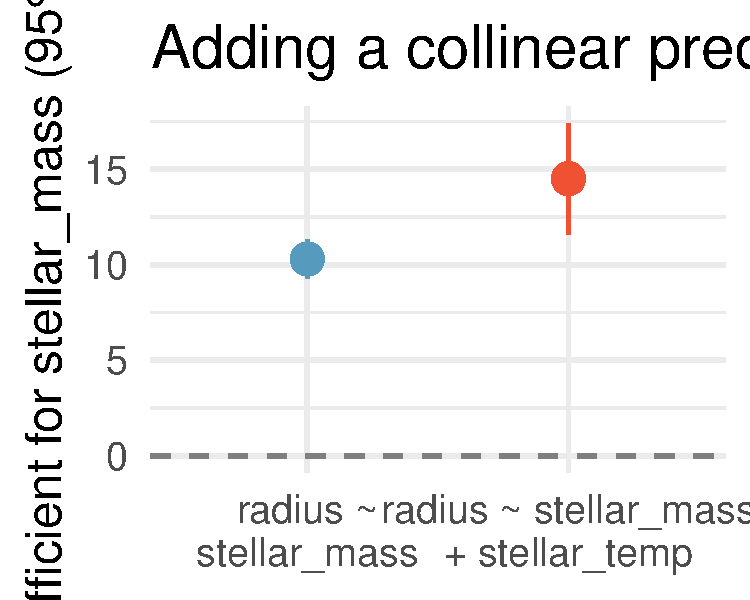
\includegraphics[width=\textwidth]{multicollinearity_coef.pdf}
\end{center}
\end{column}
\begin{column}{0.54\textwidth}
{\small The \emph{same} predictor, \texttt{stellar\_mass}, in two models:

\smallskip
\begin{tabular}{@{}lrr@{}}
\toprule
model & est. & SE \\
\midrule
$\sim$ mass & $10.30$ & $0.52$ \\
$\sim$ mass $+$ temp & $14.51$ & $\mathbf{1.48}$ \\
\bottomrule
\end{tabular}

\pause
\smallskip
Adding its twin inflates the SE by \hl{$184\%$} and makes the interval \hl{$2.8\times$ wider}. The estimate moves too.}
\end{column}
\end{columns}

\pause
\vspace{0.2em}
{\small The data cannot separate the credit due to each, so the interval stays wide. A wide interval is the honest answer here.}

\end{frame}


%%%%%%%%%%%%%%%%%%%%%%%%%%%%%%%%%%%%%%%%%%%%%%%%%%%%%%%%%%%%%%%%%%%%%%%%
\begin{frame}
\frametitle{Prediction survives; interpretation does not}

Adding the collinear twin barely changed how well the model \emph{fits}: $R^2$ went from $0.305$ to $0.312$. It wrecked only our ability to say \emph{which} star property matters.

\pause
\vspace{0.4em}
\keyidea{Collinearity is a problem for \hl{inference}, not for \hl{prediction}. If you only want $\hat y$, leave the correlated predictors in, because the fitted values are fine. If you want to interpret a coefficient, or test it, drop one of the twins or combine them, and say that you did.}

\pause
\vspace{0.3em}
{\small The price of dropping one: you may throw away something genuinely predictive. There is no free lunch here, only a choice you have to make out loud.}

\end{frame}


%%%%%%%%%%%%%%%%%%%%%%%%%%%%%%%%%%%%%%%%%%%%%%%%%%%%%%%%%%%%%%%%%%%%%%%%
\section{Checking the conditions}
%%%%%%%%%%%%%%%%%%%%%%%%%%%%%%%%%%%%%%%%%%%%%%%%%%%%%%%%%%%%%%%%%%%%%%%%
\begin{frame}[fragile]
\frametitle{LINE, in $p$ dimensions}

The $t$ model for every row in that table rests on the same \hl{LINE} conditions as Lecture 13, read off the same two plots.

\begin{Verbatim}[fontsize=\scriptsize]
plot(fit, which = 1)   # residuals vs fitted -- L and E
plot(fit, which = 2)   # normal Q-Q          -- N
\end{Verbatim}

\pause
\vspace{-0.4em}
\twocol{0.5}{0.5}
{
\begin{center}
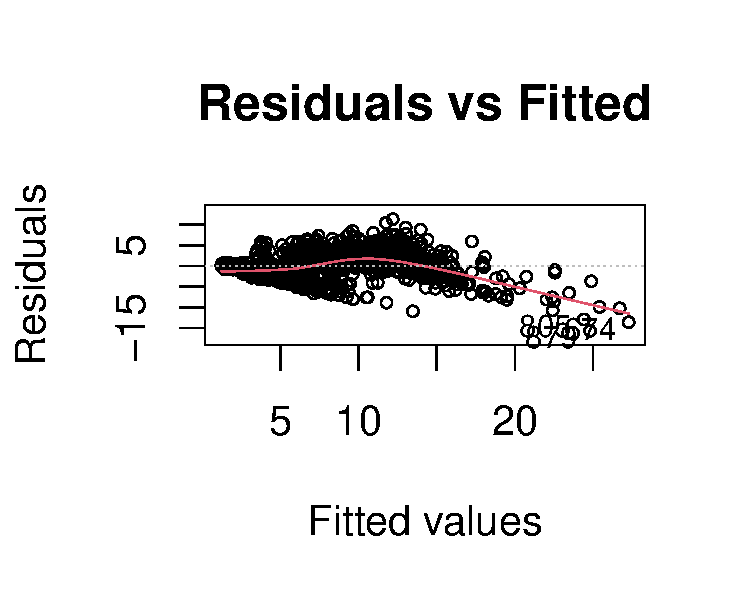
\includegraphics[width=\textwidth]{resid_vs_fitted_exo.pdf}
\end{center}
}
{
\begin{center}
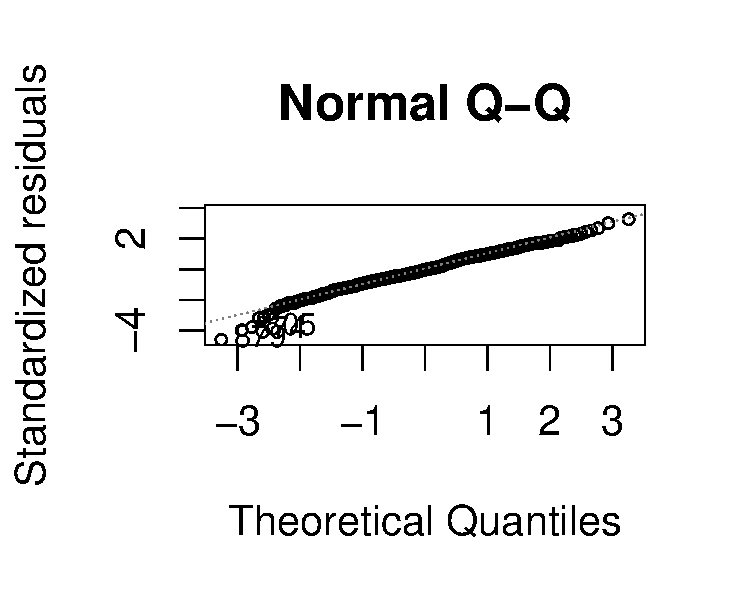
\includegraphics[width=\textwidth]{qq_exo.pdf}
\end{center}
}

\end{frame}


%%%%%%%%%%%%%%%%%%%%%%%%%%%%%%%%%%%%%%%%%%%%%%%%%%%%%%%%%%%%%%%%%%%%%%%%
\begin{frame}
\frametitle{And one plot per predictor}

A curve can hide in \emph{one} predictor while the overall residual plot looks fine. So plot residuals against each predictor:

\vspace{-0.1em}
\begin{center}
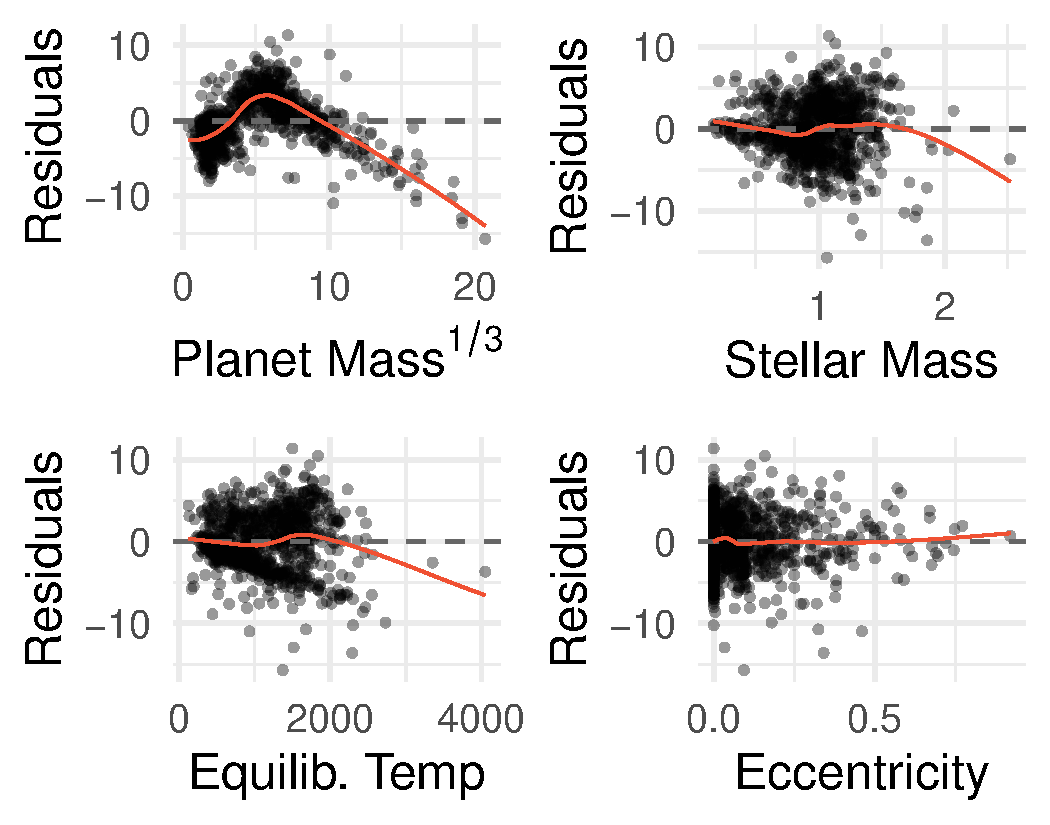
\includegraphics[width=0.52\textwidth]{resid_vs_predictors_exo.pdf}
\end{center}

\pause
\vspace{-0.5em}
{\small The fit fans out and the Q--Q tail is heavy, so \hl{those intervals are not yet trustworthy}.}

\end{frame}


%%%%%%%%%%%%%%%%%%%%%%%%%%%%%%%%%%%%%%%%%%%%%%%%%%%%%%%%%%%%%%%%%%%%%%%%
\section{Transformations and non-linear models}
%%%%%%%%%%%%%%%%%%%%%%%%%%%%%%%%%%%%%%%%%%%%%%%%%%%%%%%%%%%%%%%%%%%%%%%%
\begin{frame}
\frametitle{A line that has no business being straight}

Same planets, two other columns: a planet's \texttt{orbital\_period} against its \texttt{semi\_major\_axis}. One predictor, so the problem shows cleanly.

\vspace{0.2em}
\twocol{0.48}{0.48}{
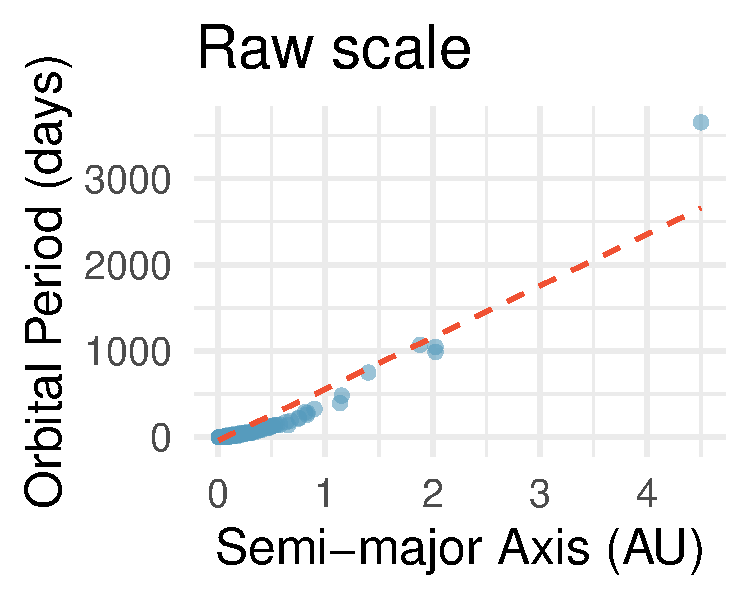
\includegraphics[width=0.95\textwidth]{period_vs_axis_raw.pdf}
}{
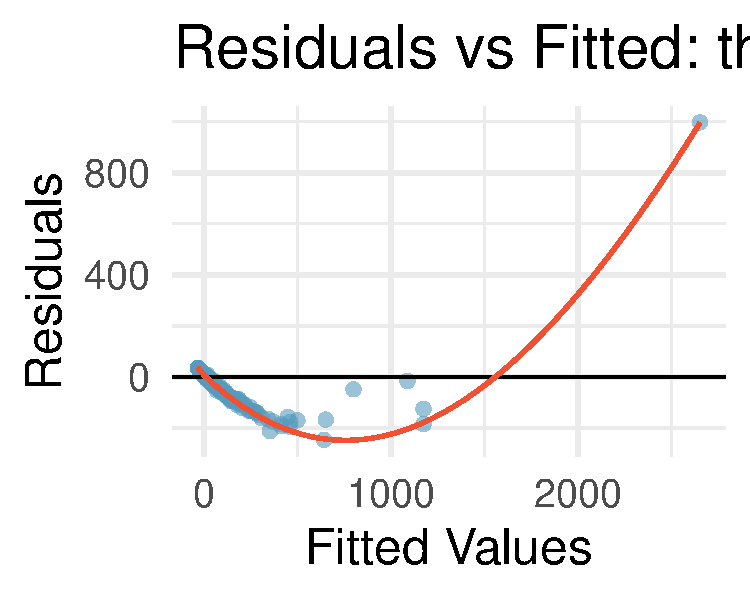
\includegraphics[width=0.95\textwidth]{period_vs_axis_residuals.pdf}
}

\pause
\vspace{-0.2em}
\dq{The line has $R^2 = 0.88$. Why is the residual plot still damning?}

\end{frame}


%%%%%%%%%%%%%%%%%%%%%%%%%%%%%%%%%%%%%%%%%%%%%%%%%%%%%%%%%%%%%%%%%%%%%%%%
\begin{frame}
\frametitle{Kepler's third law}

\twocol{0.55}{0.45}{
\begin{center}
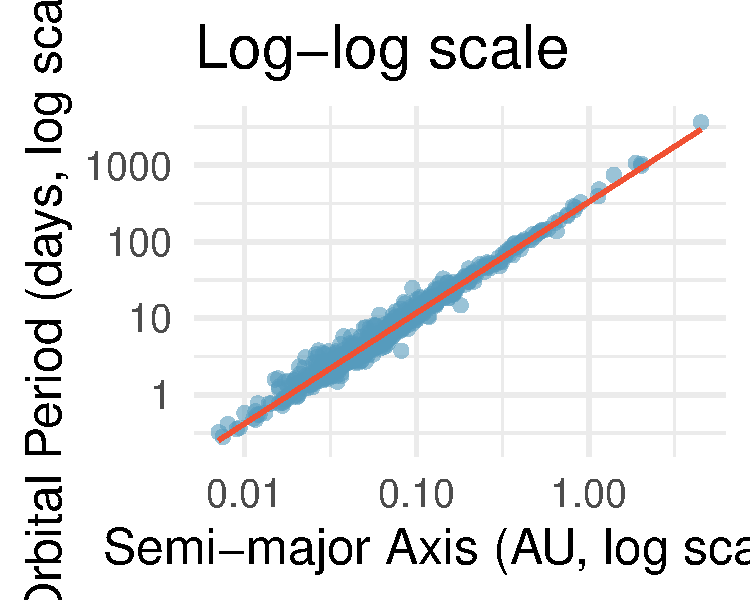
\includegraphics[width=\textwidth]{period_vs_axis_loglog.pdf}
\end{center}
}{
Plot both axes on a log scale and the curve becomes a line.

\vspace{0.5em}
\textbf{Kepler's third law:} $P^2 \propto a^3$.

\vspace{0.4em}
Take logs of both sides:
$$\log P \approx \tfrac{3}{2}\,\log a + c$$

\vspace{0.3em}
A \hl{power law in the raw variables is a straight line in the logs}, and a straight line is something we know how to fit, test and bound.
}

\end{frame}


%%%%%%%%%%%%%%%%%%%%%%%%%%%%%%%%%%%%%%%%%%%%%%%%%%%%%%%%%%%%%%%%%%%%%%%%
\begin{frame}[fragile]
\frametitle{Fitting it, and reading the slope}

\begin{Verbatim}[fontsize=\scriptsize]
loglog <- lm(log(orbital_period) ~ log(semi_major_axis),
             data = exo)
loglog |> tidy(conf.int = TRUE)

  term                  estimate  std.error  conf.low  conf.high
  (Intercept)             5.804     0.022      5.761     5.848
  log(semi_major_axis)    1.450     0.008      1.435     1.465
\end{Verbatim}

\pause
\vspace{0.2em}
$R^2$ climbs from $0.88$ to $0.976$, and $\hat\beta_1 = 1.450$ sits a whisker from Kepler's $3/2$.

\pause
\vspace{0.3em}
\dq{But the 95\% interval is $(1.435,\ 1.465)$, which \emph{excludes} $1.5$. Have we just refuted Kepler?}

\end{frame}


%%%%%%%%%%%%%%%%%%%%%%%%%%%%%%%%%%%%%%%%%%%%%%%%%%%%%%%%%%%%%%%%%%%%%%%%
\begin{frame}
\frametitle{Did the transformation fix the diagnostics?}

\begin{center}
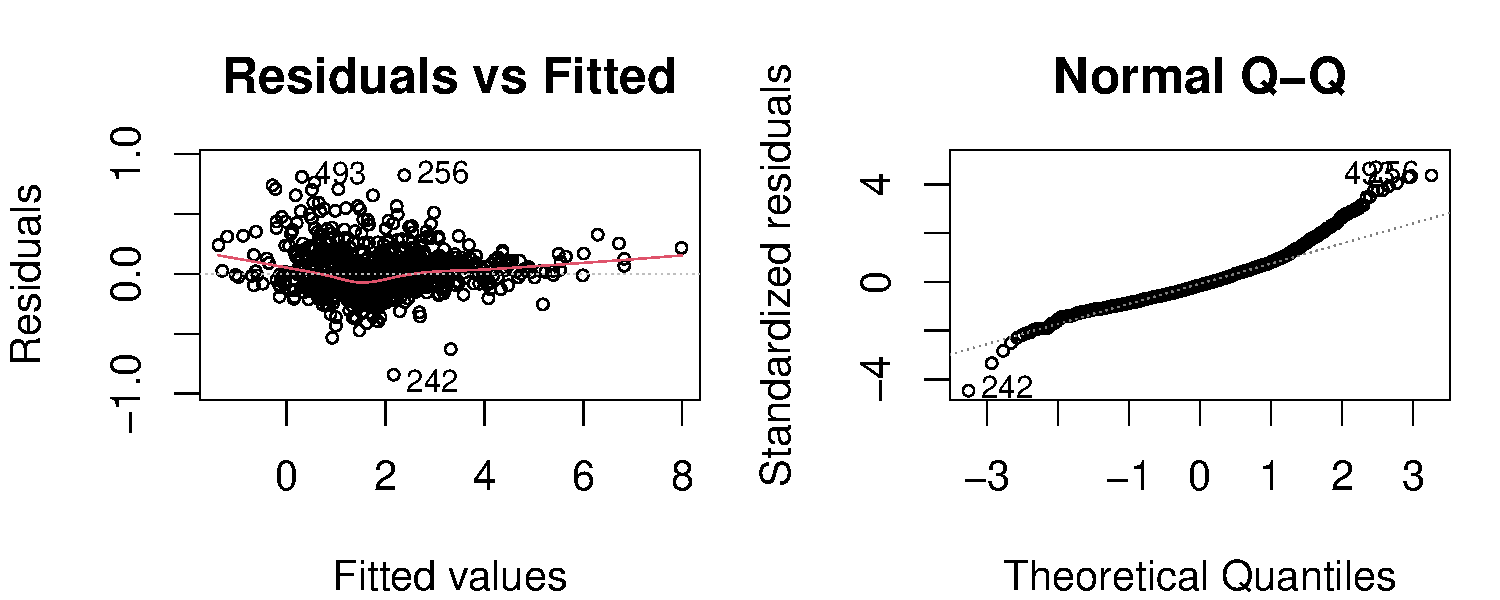
\includegraphics[width=0.93\textwidth]{loglog_diagnostics.pdf}
\end{center}

\pause
\vspace{-0.2em}
{\small \hl{The curvature is gone} after the transformation. But the tails are still heavy, so the $t$ model behind that narrow interval is not on solid ground. Before believing an interval that excludes $1.5$, get a second opinion.}

\end{frame}


%%%%%%%%%%%%%%%%%%%%%%%%%%%%%%%%%%%%%%%%%%%%%%%%%%%%%%%%%%%%%%%%%%%%%%%%
\begin{frame}
\frametitle{The two roads, one more time}

\twocol{0.55}{0.45}{
\begin{center}
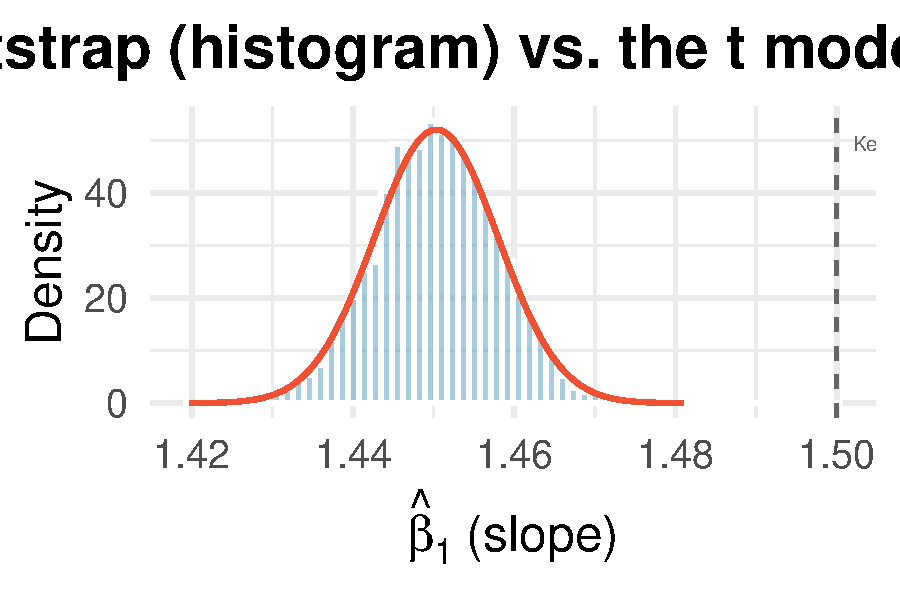
\includegraphics[width=\textwidth]{loglog_bootstrap_vs_model.pdf}
\end{center}
}{
{\small \hl{Bootstrap the pairs:} CI $(1.435,\ 1.465)$.

\smallskip
\hl{The $t$ formula:} CI $(1.435,\ 1.465)$.

\smallskip
The histogram and the curve lie on top of each other. The interval is \emph{not} an artefact of a shaky $t$ approximation: both roads exclude $1.5$.}
}

\pause
\vspace{-0.2em}
{\small So the narrowness is real, and the answer to ``have we refuted Kepler?'' is \hl{no: we have caught our own model}. Kepler's constant depends on the star's mass, and we pooled planets orbiting stars of quite different masses. A missing predictor, not a broken law.}

\end{frame}


%%%%%%%%%%%%%%%%%%%%%%%%%%%%%%%%%%%%%%%%%%%%%%%%%%%%%%%%%%%%%%%%%%%%%%%%
\begin{frame}
\frametitle{Three ways a model can be wrong}

\keyidea{A transformation can remedy three failures a residual plot shows:
\begin{itemize}\setlength{\itemsep}{1pt}
\item \hl{non-linearity}: a curve in residuals vs.\ fitted;
\item \hl{non-constant variance}: a fan or funnel;
\item \hl{non-normal errors}: a bent Q--Q plot.
\end{itemize}
Diagnose first, and transform only when the new model still makes scientific sense.}

\pause
\vspace{0.3em}
First ask whether a transformation has a sensible interpretation, then \hl{which variable}, $y$ or $x$. Simulated data settles the second: we know the true model.

\end{frame}


%%%%%%%%%%%%%%%%%%%%%%%%%%%%%%%%%%%%%%%%%%%%%%%%%%%%%%%%%%%%%%%%%%%%%%%%
\begin{frame}
\frametitle{A funnel: transform $y$, not $x$}

Truth: $\log(y) = 2 + 0.5x + \varepsilon$. The errors are multiplicative on the raw scale, so the spread grows with $y$.

\vspace{0.2em}
\begin{center}
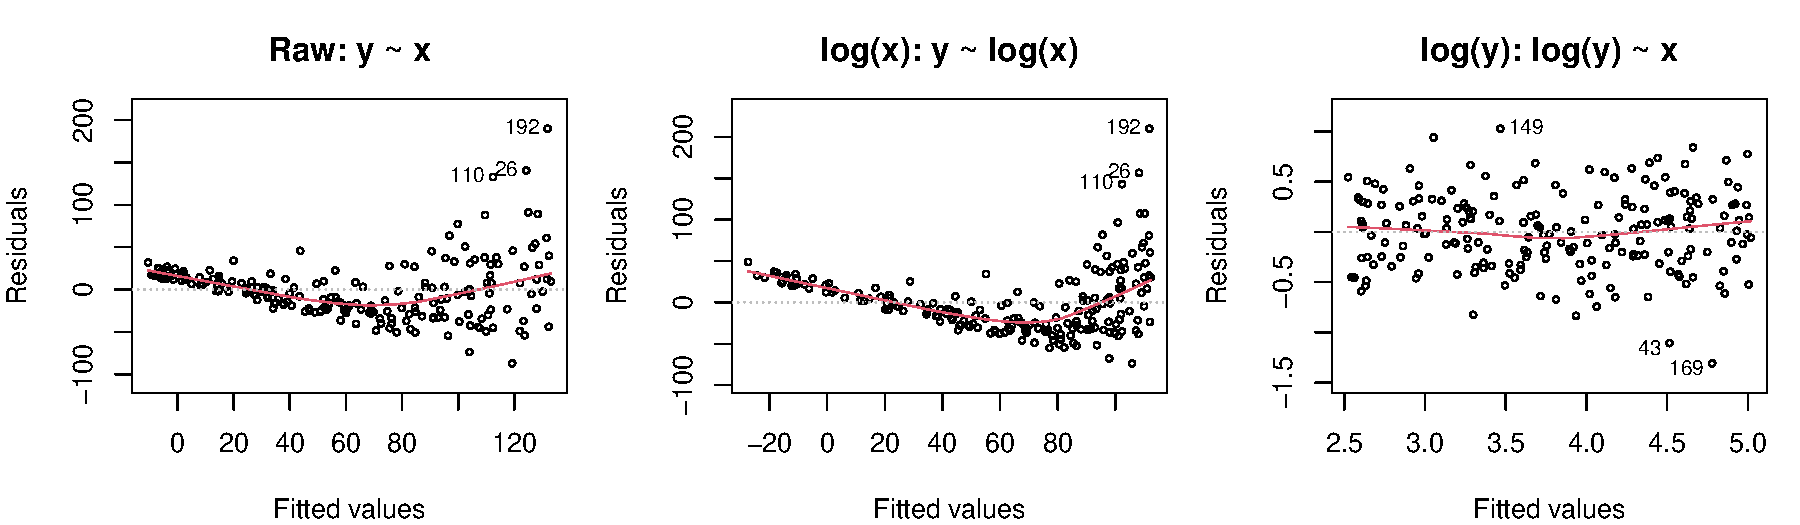
\includegraphics[width=\textwidth]{synth_hetero.pdf}
\end{center}

\pause
\vspace{-0.3em}
{\small Funnel score $\mathrm{cor}(|e|,\hat y)$: raw $0.46$, $\log(x)$ $0.34$, $\log(y)$ $\mathbf{0.07}$. \hl{Only transforming $y$ flattens it}-- bending the $x$-axis cannot fix a problem that lives in $y$.}

\end{frame}


%%%%%%%%%%%%%%%%%%%%%%%%%%%%%%%%%%%%%%%%%%%%%%%%%%%%%%%%%%%%%%%%%%%%%%%%
\begin{frame}
\frametitle{A bent Q--Q plot: transform $y$, not $x$}

The same simulated data, now judged by the Q--Q plot:

\vspace{0.2em}
\begin{center}
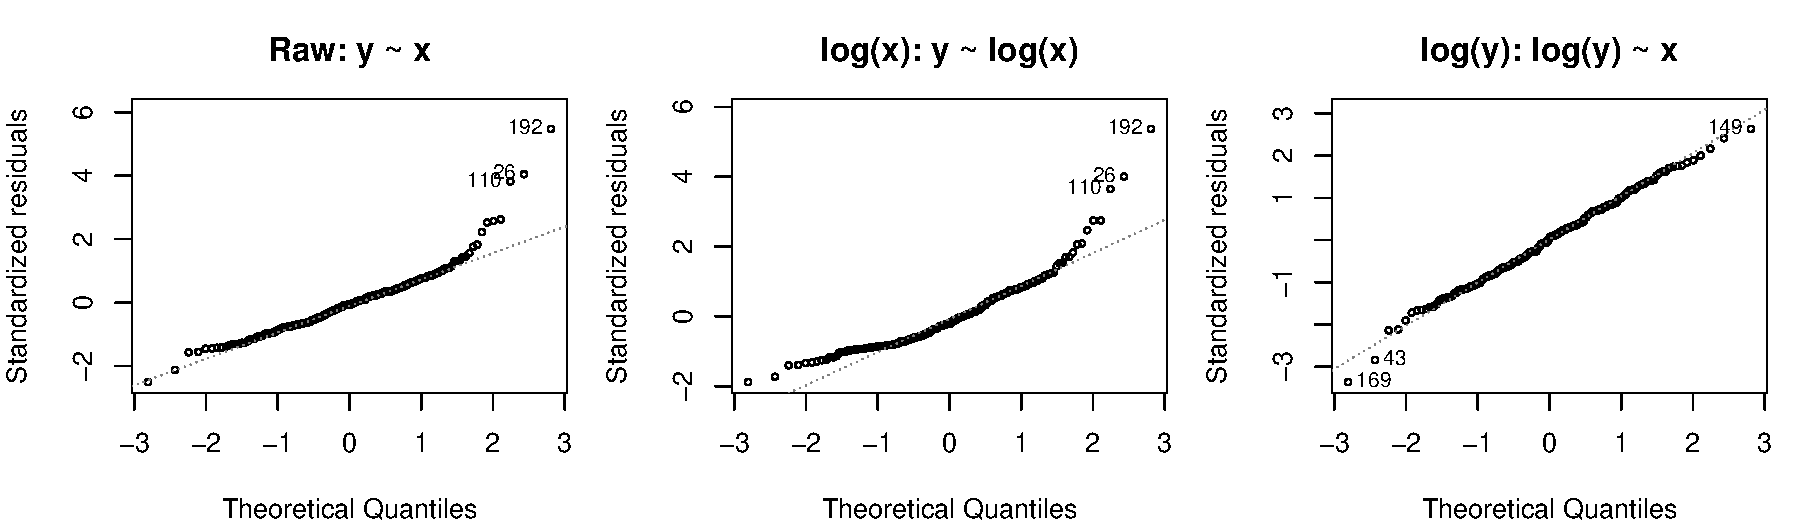
\includegraphics[width=\textwidth]{synth_nonnormal.pdf}
\end{center}

\pause
\vspace{-0.3em}
{\small Raw and $\log(x)$ have the same heavy right tail, unsurprising since they have the \emph{same} response. $\log(y)$ puts the points back on the line. \hl{Equal variance and normality are properties of the errors, so they are fixed on the $y$ side.}}

\end{frame}


%%%%%%%%%%%%%%%%%%%%%%%%%%%%%%%%%%%%%%%%%%%%%%%%%%%%%%%%%%%%%%%%%%%%%%%%
\begin{frame}
\frametitle{A curve: it depends on the curve}

\begin{center}
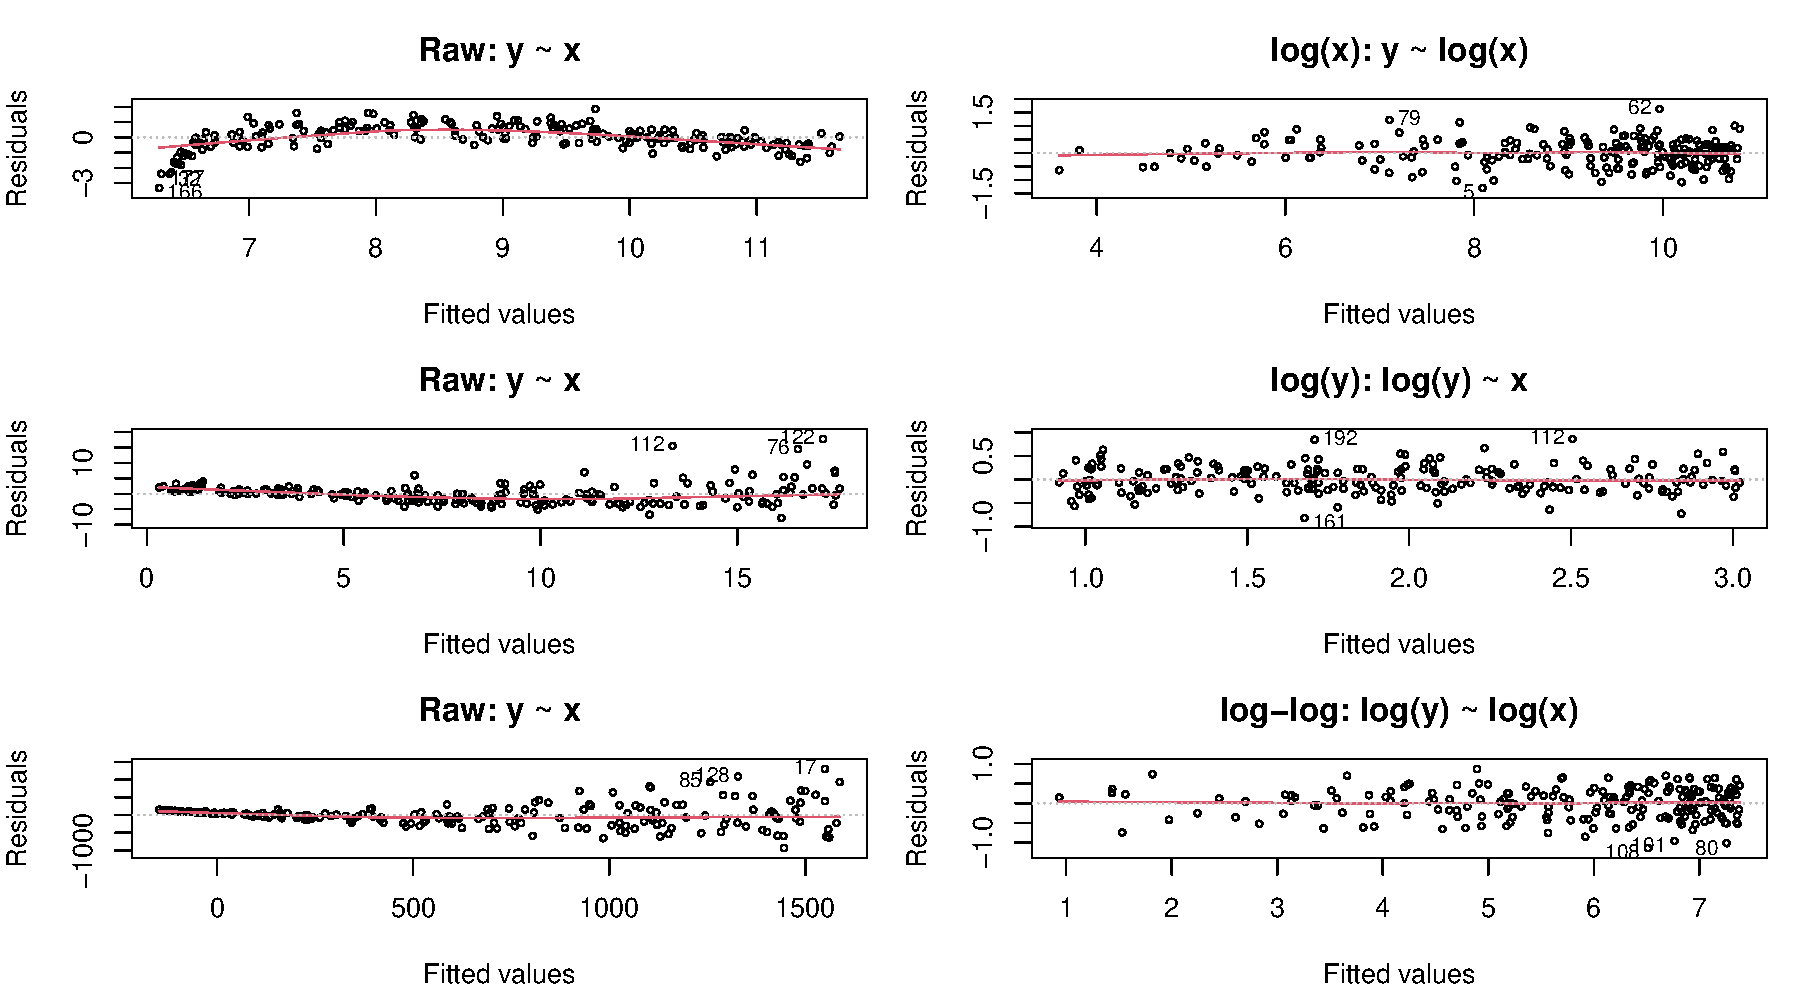
\includegraphics[width=0.86\textwidth]{synth_nonlinear.pdf}
\end{center}

\pause
\vspace{-0.3em}
{\small Three curves, three repairs: diminishing returns takes $\log(x)$, exponential growth $\log(y)$, a power law \emph{both}. \hl{Try one and read the residual plot.}}

\end{frame}


%%%%%%%%%%%%%%%%%%%%%%%%%%%%%%%%%%%%%%%%%%%%%%%%%%%%%%%%%%%%%%%%%%%%%%%%
\begin{frame}
\frametitle{What a log-log slope means}
$$\log(y) = \hat\beta_0 + \hat\beta_1 \log(x) \qquad\Longleftrightarrow\qquad y = e^{\hat\beta_0} \cdot x^{\hat\beta_1}$$

\pause
\vspace{0.3em}
Multiply $x$ by $k$, and $y$ is multiplied by $k^{\hat\beta_1}$:
$$e^{\hat\beta_0}(kx)^{\hat\beta_1} = k^{\hat\beta_1}\cdot e^{\hat\beta_0}x^{\hat\beta_1} = k^{\hat\beta_1}\, y$$

\pause
\vspace{0.3em}
\formula{Power law}{A log--log slope is an \hl{elasticity}: a $1\%$ increase in $x$ gives about a $\hat\beta_1\%$ increase in $y$. For Kepler, $\hat\beta_1 = 1.45$: move a planet twice as far out and its year gets $2^{1.45} \approx 2.7$ times longer.}

\end{frame}


%%%%%%%%%%%%%%%%%%%%%%%%%%%%%%%%%%%%%%%%%%%%%%%%%%%%%%%%%%%%%%%%%%%%%%%%
\begin{frame}
\frametitle{The three logs, side by side}

{\footnotesize
\begin{center}
\setlength{\tabcolsep}{4pt}
\renewcommand{\arraystretch}{1.4}
\begin{tabular}{@{}lll@{}}
\toprule
\textbf{Model} & \textbf{Back-transformed} & \textbf{Changing $x$} \\
\midrule
$\log y = \beta_0 + \beta_1 x$ & $y = e^{\beta_0}e^{\beta_1 x}$ (exponential) & $+1$ in $x$ \emph{multiplies} $y$ by $e^{\beta_1}$ \\
$y = \beta_0 + \beta_1 \log x$ & n/a (already in $y$) & doubling $x$ adds $0.69\,\beta_1$ to $y$ \\
$\log y = \beta_0 + \beta_1 \log x$ & $y = e^{\beta_0} x^{\beta_1}$ (power law) & doubling $x$ multiplies $y$ by $2^{\beta_1}$ \\
\bottomrule
\end{tabular}
\end{center}}

\pause
\vspace{0.2em}
{\small \textbf{Worked example ($\log y$).} If $\hat\beta_1 = 0.05$, then each one-unit rise in $x$ multiplies $y$ by $e^{0.05} \approx 1.05$, about a $5\%$ increase. That shortcut, $100\hat\beta_1\%$, is good only while $|\hat\beta_1|$ is small.}

\pause
\vspace{0.2em}
{\small And note what does \emph{not} change: \hl{the inference is untouched}. The $t$ test, the interval, the LINE checks all apply to the transformed model exactly as before. Only the \emph{sentence you say out loud} about $\hat\beta_1$ changes.}

\end{frame}


%%%%%%%%%%%%%%%%%%%%%%%%%%%%%%%%%%%%%%%%%%%%%%%%%%%%%%%%%%%%%%%%%%%%%%%%
\begin{frame}
\frametitle{The radius: cube root, or logs?}

Two ways to straighten radius against mass. Which should we keep?

\pause
\vspace{0.2em}
\begin{center}
{\small
\begin{tabular}{@{}lccc@{}}
\toprule
\textbf{Model} & \textbf{Adj.\ $R^2$} & \textbf{AIC} & \textbf{Funnel score} \\
\midrule
$\text{radius} \sim \text{mass}^{1/3}$ & $0.520$ & $4961$ & $0.36$ \\
$\log(\text{radius}) \sim \log(\text{mass})$ & $0.776$ & $1022$ & $0.16$ \\
\bottomrule
\end{tabular}}
\end{center}

\pause
\vspace{0.2em}
\caution{Do \emph{not} read that AIC column. AIC and $R^2$ compare models with the \hl{same response}, but here one predicts \texttt{radius} and the other $\log(\texttt{radius})$. Judge these two by their \hl{diagnostics}.}

\end{frame}


%%%%%%%%%%%%%%%%%%%%%%%%%%%%%%%%%%%%%%%%%%%%%%%%%%%%%%%%%%%%%%%%%%%%%%%%
\begin{frame}
\frametitle{Choosing between them on the residuals}

\textbf{Cube root:} $\text{radius} \sim \text{mass}^{1/3}$
\begin{center}
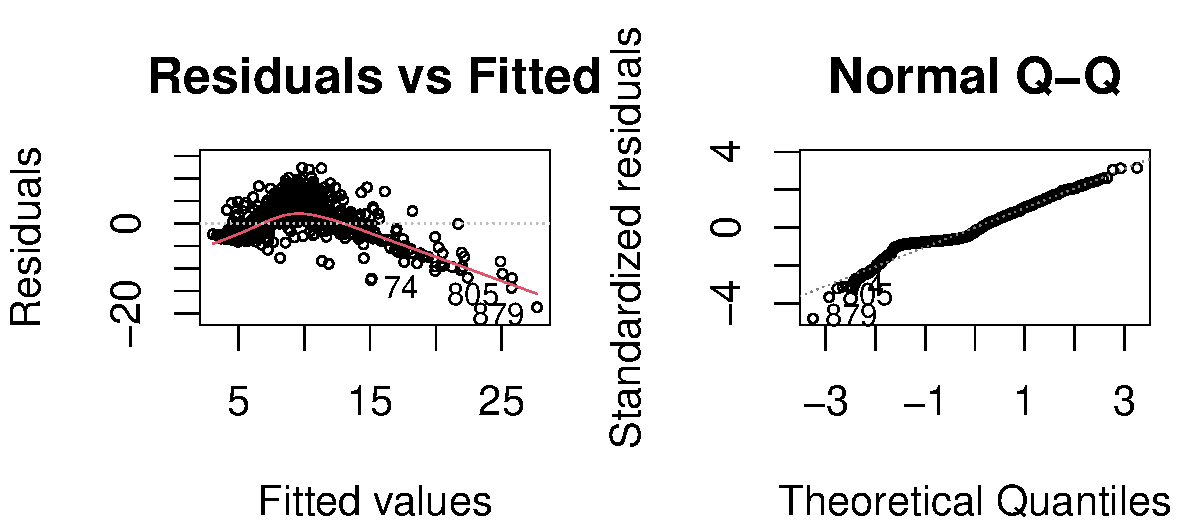
\includegraphics[width=0.86\linewidth]{radius_cbrtmass_diagnostics.pdf}
\end{center}

\vspace{-0.2em}
{\small A clear arch remains in the residuals: the cube root has not straightened it.}

\end{frame}

%%%%%%%%%%%%%%%%%%%%%%%%%%%%%%%%%%%%%%%%%%%%%%%%%%%%%%%%%%%%%%%%%%%%%%%%
\begin{frame}
\frametitle{Choosing between them: the log--log residuals}

\textbf{Log--log:} $\log(\text{radius}) \sim \log(\text{mass})$
\begin{center}
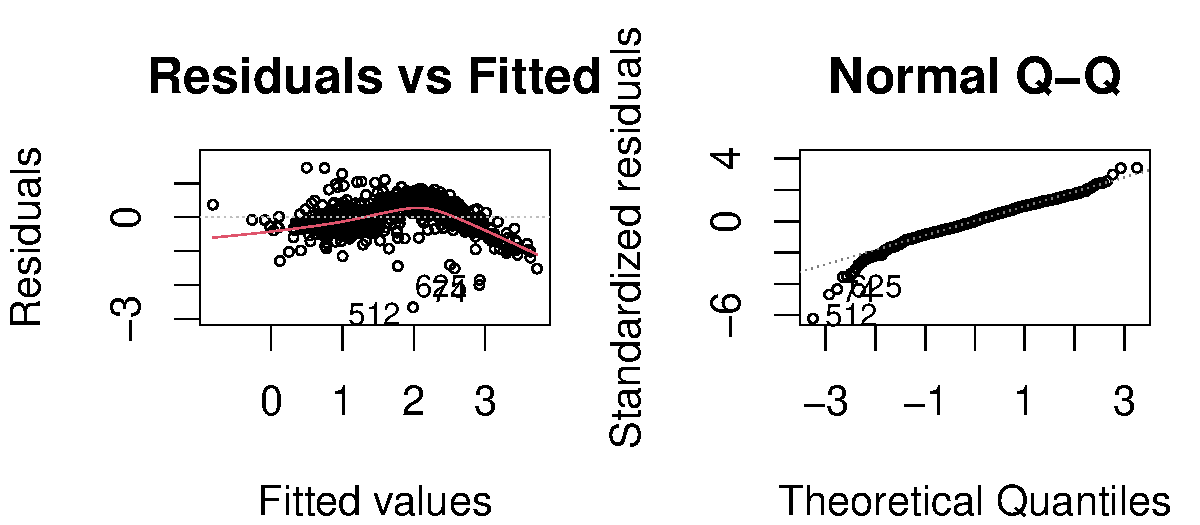
\includegraphics[width=0.86\linewidth]{radius_loglog_diagnostics.pdf}
\end{center}

\vspace{-0.2em}
{\small Flatter and more even, so the log--log fit is the one to keep.}

\end{frame}


%%%%%%%%%%%%%%%%%%%%%%%%%%%%%%%%%%%%%%%%%%%%%%%%%%%%%%%%%%%%%%%%%%%%%%%%
\section{Interaction terms}
%%%%%%%%%%%%%%%%%%%%%%%%%%%%%%%%%%%%%%%%%%%%%%%%%%%%%%%%%%%%%%%%%%%%%%%%
\begin{frame}
\frametitle{When a slope depends on another predictor}

In Lecture 5 we fitted two groups with a shared slope, so the lines were \emph{forced} to stay parallel. An \hl{interaction} lets that slope change:
$$y = \beta_0 + \beta_1 x_1 + \beta_2 x_2 + \beta_3\,(x_1 \cdot x_2)$$

\pause
\vspace{0.3em}
Collect the terms that multiply $x_1$:
$$y = \underbrace{(\beta_0 + \beta_2 x_2)}_{\text{intercept}} \;+\; \underbrace{(\beta_1 + \beta_3 x_2)}_{\text{slope of } x_1} \cdot\, x_1$$

\pause
\vspace{0.3em}
\formula{Reading $\beta_3$}{Fix $x_2$ and you still have a straight line in $x_1$, but its \hl{slope now moves with $x_2$}, by $\beta_3$ per unit of $x_2$. $\beta_3 = 0$ is the parallel-lines model we have been fitting all along.}

\end{frame}


%%%%%%%%%%%%%%%%%%%%%%%%%%%%%%%%%%%%%%%%%%%%%%%%%%%%%%%%%%%%%%%%%%%%%%%%
\begin{frame}[fragile]
\frametitle{The books, with an interaction}

Lecture 5's $15$ books. Cover type entered as an indicator, and the two fitted lines came out \hl{parallel by construction}, same slope $0.72$ g/cm$^3$, paperbacks sitting $184$ g lower:
$$\widehat{\text{weight}} = 197.96 + 0.72\,\text{volume} - 184.05\,\text{cover:pb}$$

\pause
\vspace{0.3em}
We never asked whether they \emph{wanted} to be parallel. One character in the formula lets us:

\begin{Verbatim}[fontsize=\scriptsize]
lm(weight ~ volume * cover, data = books)   # was: +
\end{Verbatim}

\end{frame}


%%%%%%%%%%%%%%%%%%%%%%%%%%%%%%%%%%%%%%%%%%%%%%%%%%%%%%%%%%%%%%%%%%%%%%%%
\begin{frame}
\frametitle{Two lines, no longer forced together}

\twocol{0.52}{0.48}{
\begin{center}
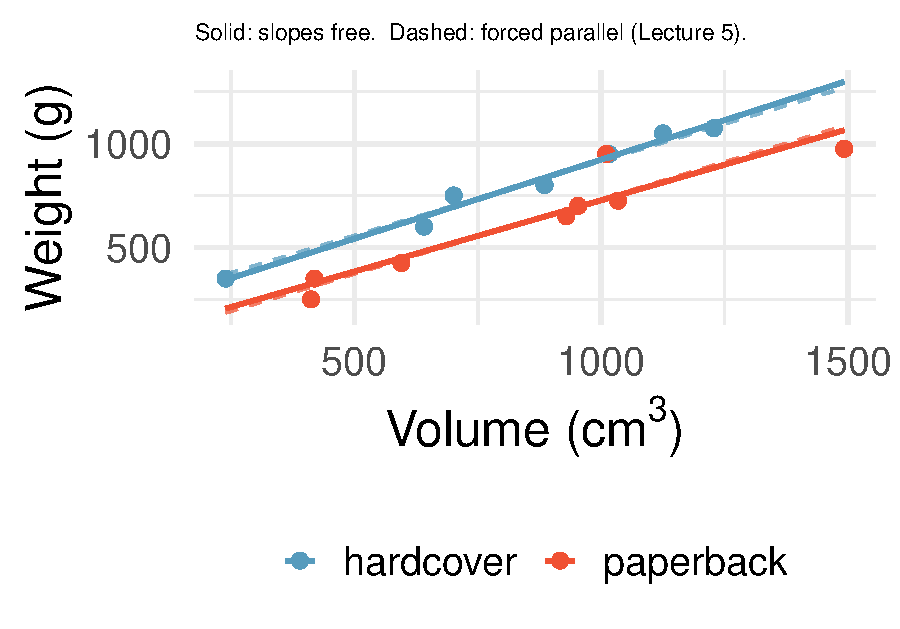
\includegraphics[width=\textwidth]{books_interaction.pdf}
\end{center}
}{
{\small
Set \texttt{cover:pb} to $0$ and to $1$, as in Lecture 5, but now the interaction rides along:

\smallskip
\hl{Hardcover:} $\widehat{w} = 161.6 + 0.762\,v$

\smallskip
\hl{Paperback:} $\widehat{w} = 41.4 + 0.686\,v$

\smallskip
The slopes are free, and they \emph{did} come apart: $0.762$ vs.\ $0.686$.}
}

\pause
\vspace{-0.2em}
\dq{The solid lines are no longer parallel. Have we just shown that paperbacks gain weight more slowly than hardcovers?}

\end{frame}


%%%%%%%%%%%%%%%%%%%%%%%%%%%%%%%%%%%%%%%%%%%%%%%%%%%%%%%%%%%%%%%%%%%%%%%%
\begin{frame}[fragile]
\frametitle{No. Look at the row.}

\begin{Verbatim}[fontsize=\scriptsize]
  term                    estimate  std.error  statistic  p.value
  volume                     0.762     0.097      7.84     <0.001
  cover:pb                -120.214   115.659     -1.04      0.321
  volume:cover:pb           -0.076     0.128     -0.59      0.566
\end{Verbatim}

\pause
\vspace{0.2em}
{\small $\hat\beta_3 = -0.076$ with $\mathrm{SE} = 0.128$: the gap between the two slopes is smaller than its own noise ($p = 0.566$). The extra parameter makes the model \emph{worse}: adjusted $R^2$ $0.915 \to 0.911$, AIC $178.0 \to 179.5$.}

\pause
\vspace{0.2em}
\keyidea{An interaction is a \hl{claim you test}, not a decoration you add. Here the data did not support it: Lecture 5's parallel-slopes model was right about these books. Two lines that \emph{look} different on a plot of $15$ points are not two different lines.}

\end{frame}


%%%%%%%%%%%%%%%%%%%%%%%%%%%%%%%%%%%%%%%%%%%%%%%%%%%%%%%%%%%%%%%%%%%%%%%%
\begin{frame}[fragile]
\frametitle{Does the star bend the mass--radius law?}

Now a \emph{numerical} $x_2$. The algebra is identical, only \texttt{cover:pb} becomes a number that varies continuously. And this time it is the loose end from Kepler: the mass--radius relation may not be the same around every star.

\begin{Verbatim}[fontsize=\scriptsize]
lm(log(planet_radius) ~ log(planet_mass) * stellar_mass)

  term                            estimate  std.error  p.value
  (Intercept)                      -0.430     0.093     <0.001
  log(planet_mass)                  0.468     0.021     <0.001
  stellar_mass                      0.821     0.108     <0.001
  log(planet_mass):stellar_mass    -0.113     0.021     <0.001
\end{Verbatim}

\pause
\vspace{0.2em}
{\small $\hat\beta_3 = -0.113$, and it is nowhere near zero ($p < 0.001$). The parallel-lines model is \hl{rejected}.}

\end{frame}


%%%%%%%%%%%%%%%%%%%%%%%%%%%%%%%%%%%%%%%%%%%%%%%%%%%%%%%%%%%%%%%%%%%%%%%%
\begin{frame}
\frametitle{What $\hat\beta_3 = -0.113$ actually says}
$$\text{slope of } \log(\text{mass}) \;=\; 0.468 \;-\; 0.113 \cdot \texttt{stellar\_mass}$$

\pause
\vspace{0.2em}
\twocol{0.52}{0.48}{
\begin{center}
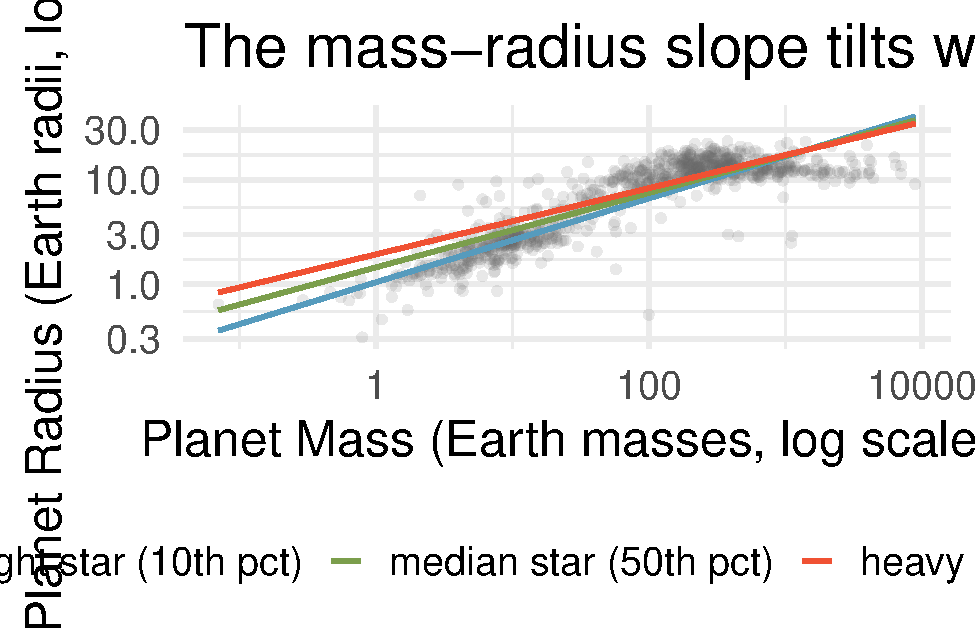
\includegraphics[width=\textwidth]{interaction_effect.pdf}
\end{center}
}{
{\small
\begin{tabular}{@{}lc@{}}
\toprule
host star & slope \\
\midrule
light ($0.58 M_\odot$) & $0.402$ \\
median ($0.98 M_\odot$) & $0.357$ \\
heavy ($1.33 M_\odot$) & $0.317$ \\
\bottomrule
\end{tabular}

\smallskip
Around \emph{heavier} stars, the same extra mass buys a planet \hl{less} extra radius, so the mass--radius law is flatter.}
}

\end{frame}


%%%%%%%%%%%%%%%%%%%%%%%%%%%%%%%%%%%%%%%%%%%%%%%%%%%%%%%%%%%%%%%%%%%%%%%%
\begin{frame}
\frametitle{Was it worth the extra parameter?}

All three models predict $\log(\text{radius})$ from the \emph{same} $890$ planets, so now AIC \emph{is} a fair comparison.

\pause
\vspace{0.3em}
\begin{center}
{\small
\begin{tabular}{@{}lcc@{}}
\toprule
\textbf{Model} & \textbf{Adj.\ $R^2$} & \textbf{AIC} \\
\midrule
$\log(\text{mass})$ & $0.776$ & $1022$ \\
$+\ \texttt{stellar\_mass}$ & $0.784$ & $991$ \\
$\times\ \texttt{stellar\_mass}$ (interaction) & $0.791$ & $964$ \\
\bottomrule
\end{tabular}}
\end{center}

\pause
\vspace{0.3em}
\dq{AIC drops by $27$. Is a better AIC, on its own, a good enough reason to keep a term?}

\end{frame}


%%%%%%%%%%%%%%%%%%%%%%%%%%%%%%%%%%%%%%%%%%%%%%%%%%%%%%%%%%%%%%%%%%%%%%%%
\begin{frame}
\frametitle{Keeping a term: discussion}

\emph{Is a better AIC, on its own, a good enough reason to keep a term?}

\pause
\vspace{0.5em}
\solnbox{It helps, but it is not the argument. The interaction earns its place because
\begin{itemize}\setlength{\itemsep}{1pt}
\item it is strongly supported ($p < 0.001$);
\item it has a physical meaning we can state in one sentence;
\item it explains the Kepler anomaly we had already met.
\end{itemize}
AIC is a tiebreaker, not a reason. If you cannot say \emph{what a term means}, a $\Delta$AIC of $27$ will not save you.}

\end{frame}


%%%%%%%%%%%%%%%%%%%%%%%%%%%%%%%%%%%%%%%%%%%%%%%%%%%%%%%%%%%%%%%%%%%%%%%%
\begin{frame}
\frametitle{And check it, like any other model}

Diagnostics for $\log(\text{radius}) \sim \log(\text{mass}) \times \texttt{stellar\_mass}$:

\vspace{0.4em}
\begin{center}
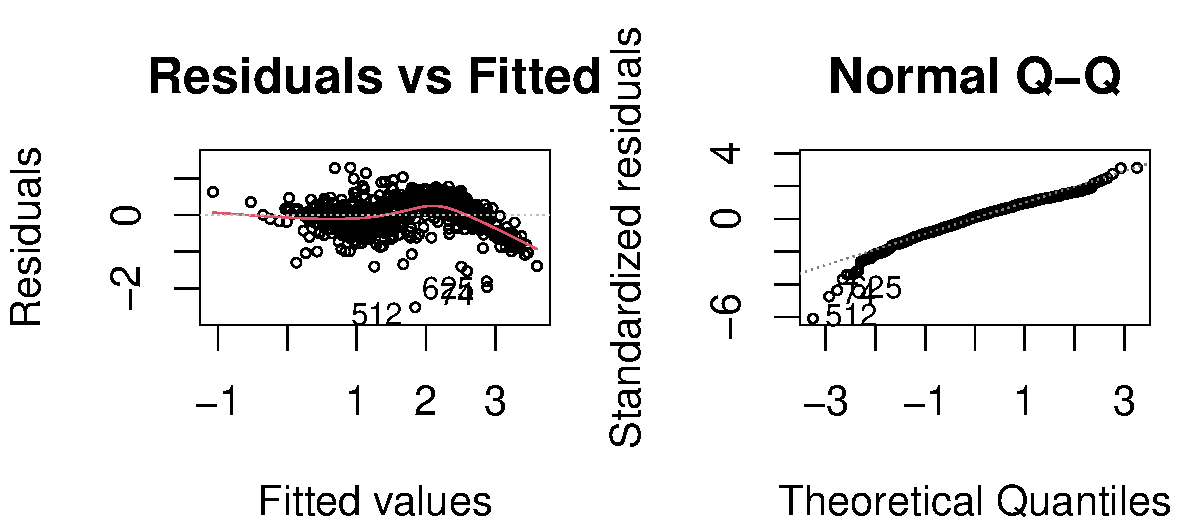
\includegraphics[width=0.72\linewidth]{radius_interaction_diagnostics.pdf}
\end{center}

\pause
\vspace{-0.2em}
{\small An interaction is not a license to skip the checks. It is just another column in the model matrix, and LINE still has to hold.}

\end{frame}


%%%%%%%%%%%%%%%%%%%%%%%%%%%%%%%%%%%%%%%%%%%%%%%%%%%%%%%%%%%%%%%%%%%%%%%%
\section{Wrap-up}
%%%%%%%%%%%%%%%%%%%%%%%%%%%%%%%%%%%%%%%%%%%%%%%%%%%%%%%%%%%%%%%%%%%%%%%%
\begin{frame}
\frametitle{The same two roads, now with $p$ predictors}

{\scriptsize
\begin{center}
\setlength{\tabcolsep}{2.5pt}
\begin{tabular}{lll}
\toprule
\textbf{The statistic} & \textbf{By simulation} & \textbf{By formula} \\
\midrule
a proportion & simulate $H_0$ (Lec 8) & binomial, exact; $z$ (Lec 10) \\
a mean or a difference & bootstrap (Lec 9), permute (Lec 8) & the CLT: $z$, $t$ (Lec 10) \\
a whole table, $X^2$ & permute one column (Lec 11) & $\chi^2_{df}$ (Lec 11) \\
several group means, $F$ & permute the labels (Lec 12) & $F_{df_1,df_2}$ (Lec 12) \\
a regression slope, $\hat\beta_1$ & shuffle / bootstrap pairs (Lec 13) & $t_{n-2}$ (Lec 13) \\
\hl{one slope of many, $\hat\beta_j$} & \hl{bootstrap the rows} & \hl{$t_{n-p-1}$ (today)} \\
\bottomrule
\end{tabular}
\end{center}}

\vspace{0.3em}
Adding predictors did not add a new idea. It added \emph{rows}, and one new sentence to say about each of them: \emph{holding the others fixed}.

\end{frame}


%%%%%%%%%%%%%%%%%%%%%%%%%%%%%%%%%%%%%%%%%%%%%%%%%%%%%%%%%%%%%%%%%%%%%%%%
\begin{frame}
\frametitle{Summary}

\begin{itemize}
\item \texttt{lm()} gives \hl{one row per coefficient}: estimate, SE, $t$, $p$-value, interval. The only thing that changed is $\mathrm{df} = n-p-1$.
\item Every row is conditional: $\hat\beta_j$ is the effect of $x_j$ \hl{holding the others fixed}, and its $p$-value depends on what else is in the model.
\item \hl{Collinearity} inflates SEs and widens intervals ($+184\%$ for our stellar twins) but leaves predictions alone. It is an inference problem, not a fitting one.
\item When LINE fails, \hl{transform}: funnels and heavy tails are fixed on the $y$ side; a curve may want either side. Then re-check.
\item A log--log slope is an \hl{elasticity}. An \hl{interaction} lets one slope depend on another predictor, and is a \hl{claim you test}: the exoplanets kept theirs ($p<0.001$), the books threw theirs away ($p=0.57$).
\end{itemize}

\end{frame}


%%%%%%%%%%%%%%%%%%%%%%%%%%%%%%%%%%%%%%%%%%%%%%%%%%%%%%%%%%%%%%%%%%%%%%%%
\begin{frame}
\frametitle{Coming up next}

\hl{Lecture 15: prediction and cross-validation.} We have spent two lectures asking whether the coefficients are real. Next we ask what the model is actually \emph{for}: predicting a new planet.

\vspace{0.4em}
\begin{itemize}
\item Two quite different intervals: one for the \hl{mean} response at a given $x$, one for an \hl{individual} new observation. (They differ by a lot, and mixing them up is a classic error.)
\item How well does a model predict data it has \emph{not} seen? \hl{Cross-validation}, and why a model that fits beautifully can predict terribly.
\end{itemize}

\vspace{0.4em}
{\small IMS Ch.\ 25, plus supplements.}

\end{frame}


%%%%%%%%%%%%%%%%%%%%%%%%%%%%%%%%%%%%%%%%%%%%%%%%%%%%%%%%%%%%%%%%%%%%%%%%
% Activity
%%%%%%%%%%%%%%%%%%%%%%%%%%%%%%%%%%%%%%%%%%%%%%%%%%%%%%%%%%%%%%%%%%%%%%%%
\begin{frame}
\frametitle{Activity: what makes a country's people live longer?}

\activity{The \emph{World Happiness Report}: $150$ countries, with life expectancy, GDP per capita, social support, freedom and more. Build a model for \texttt{life\_expectancy}:
\begin{itemize}\setlength{\itemsep}{1pt}
\item diagnose the misspecification, then transform;
\item add a predictor and test an interaction;
\item read every coefficient out loud, and decide which model you would report.
\end{itemize}}

\vspace{0.3em}
{\small
\begin{itemize}
\item Work in \emph{pairs} (analyst + guide), one worksheet per pair.
\item We pause for check-ins. \hl{Be ready to share}.
\item Data and starter code are on Blackboard.
\end{itemize}}

\end{frame}


%%%%%%%%%%%%%%%%%%%%%%%%%%%%%%%%%%%%%%%%%%%%%%%%%%%%%%%%%%%%%%%%%%%%%%%%
\begin{frame}
\frametitle{Compare with the groups around you}

\textbf{When you reach the end of Part 5:}

\vspace{0.3em}
\begin{enumerate}
\item Compare your final model with at least two neighboring pairs.
\item Did you keep the same predictors? The same transformation?
\item If not, was it a different \emph{judgment} or a different \emph{mistake}? Find out which.
\item Having heard them, would you change your model? Say why, or why not.
\end{enumerate}

\vspace{0.5em}
\hl{Write your answers in the box at the end of the worksheet.}

\end{frame}


%%%%%%%%%%%%%%%%%%%%%%%%%%%%%%%%%%%%%%%%%%%%%%%%%%%%%%%%%%%%%%%%%%%%%%%%
% End document
%%%%%%%%%%%%%%%%%%%%%%%%%%%%%%%%%%%%%%%%%%%%%%%%%%%%%%%%%%%%%%%%%%%%%%%%

\end{document}
